
\documentclass{article}
\usepackage[utf8]{inputenc}
\usepackage[titletoc, title]{appendix}
\usepackage{geometry}
\geometry{
 a4paper,
 left=27mm,
 top=30mm,
 }
\usepackage{ amssymb }
\usepackage{graphicx} % Required for the inclusion of images
\usepackage{caption}
\usepackage{subcaption}
\usepackage{amsmath} % Required for some math elements
\usepackage[labelfont=bf]{caption}



\usepackage{hyperref}
\usepackage{float}






%\setlength\parindent{0pt} % Removes all indentation from paragraphs
\usepackage{authblk}
\usepackage{wrapfig}
%\renewcommand{\labelenumi}{\alph{enumi}.} % Make numbering in the enumerate environment by letter rather than number (e.g. section 6)
\usepackage[font={small}]{caption}
%\newcommand*\diff{\mathop{}\!\mathrm{d}}
\usepackage{tikz}
\usepackage{placeins}



%----------------------------------------------------------------------------------------
%	DOCUMENT INFORMATION
%----------------------------------------------------------------------------------------

\title{Spike trains} % Title

\author{Florian \textsc{Leprévost}} % Author name

\date{\today} % Date for the report

\begin{document}
\maketitle % Insert the title, author and date

\noindent Supervisor: Manuel Beiran % Instructor/supervisor
\tableofcontents

\begin{center}
\begin{tabular}{l r}

\end{tabular}
\end{center}

%----------------------------------------------------------------------------------------
%	SECTION 0
%----------------------------------------------------------------------------------------

\section{Introduction}\label{introduction}

\indent\indent In addition to modelling behavior like learning or decision-making, it is possible to simulate neuronal activity. One can for instance simulate roughly how some neurons accumulate evidence to help make a decision with drift diffusion models, but it is also possible to have more biologically informed models. This is useful for a number of reasons in cognitive neuroscience: investigating the biophysical plausibility of computational/cognitive accounts of behavior, understanding the neurological alterations underlying (neuro-)psychological pathologies,... \\
\indent The 100 billion of neurons of our brain communicate through electro-chemical signal, via a 100 trillion connections (or synapses). Understanding this electrical activity can be quite challenging, but it is key to understand how our mind works, in health and disorder.\\

\indent Neuronal membranes are mostly impermeable - except for ionic channels - so there is a capacitance effect, \textit{i.e.} opposite charges accumulate on each side of the membrane, and a very high resistance. This makes a cell an RC circuit, which means the change in voltage doesn't follow the external current immediatly; and there is indeed a voltage difference between inside and outside the cell.\\
\indent To sum up very concisely neuronal transmission, neurons receive post-synaptic potentials (PSP) from other neurons, that transiently hyper- or de-polarize the membrane away from its equilibrium potential. If some PSP are received closely enough in time, so that the cell membrane reaches a certain threshold, some voltage-dependent channels open abruptly, and there is a sudden great depolarization, followed by a sudden hyperpolarisation back to the equilibrium potential, \textit{i.e.} an action potential (AP) or a spike. This spike then translates into PSPs in neurons that are innervated by the one having an AP (section \ref{int}).\\
\indent This is the gist of cognitive neuroscience: information is transmitted through spike trains, and is stored in the strength of connections between neurons (\textit{i.e.} synaptic weights).\\

There are several models - taking the form of differential equations - trying to describe the electrical dynamics of neurons with different levels of precision, but all try to account for the production of spikes.
%----------------------------------------------------------------------------------------
%	SECTION 1
%----------------------------------------------------------------------------------------

\section{Poisson spike trains}\label{spikes}
There is a lot of `noise' in neurons' voltage, and the emission of a spike seems rather stochastic. One reason for this is that a neuron can have thousands of connection, so that the current it receives is very noisy. The best way to approximate spike generation is to use a poisson distribition, which is the most unpredictable: the probability of generating a spike in a time bin is independent of generating a spike in another (Figure \ref{fig:fig1} Up.).

\begin{figure}[H]
\centering
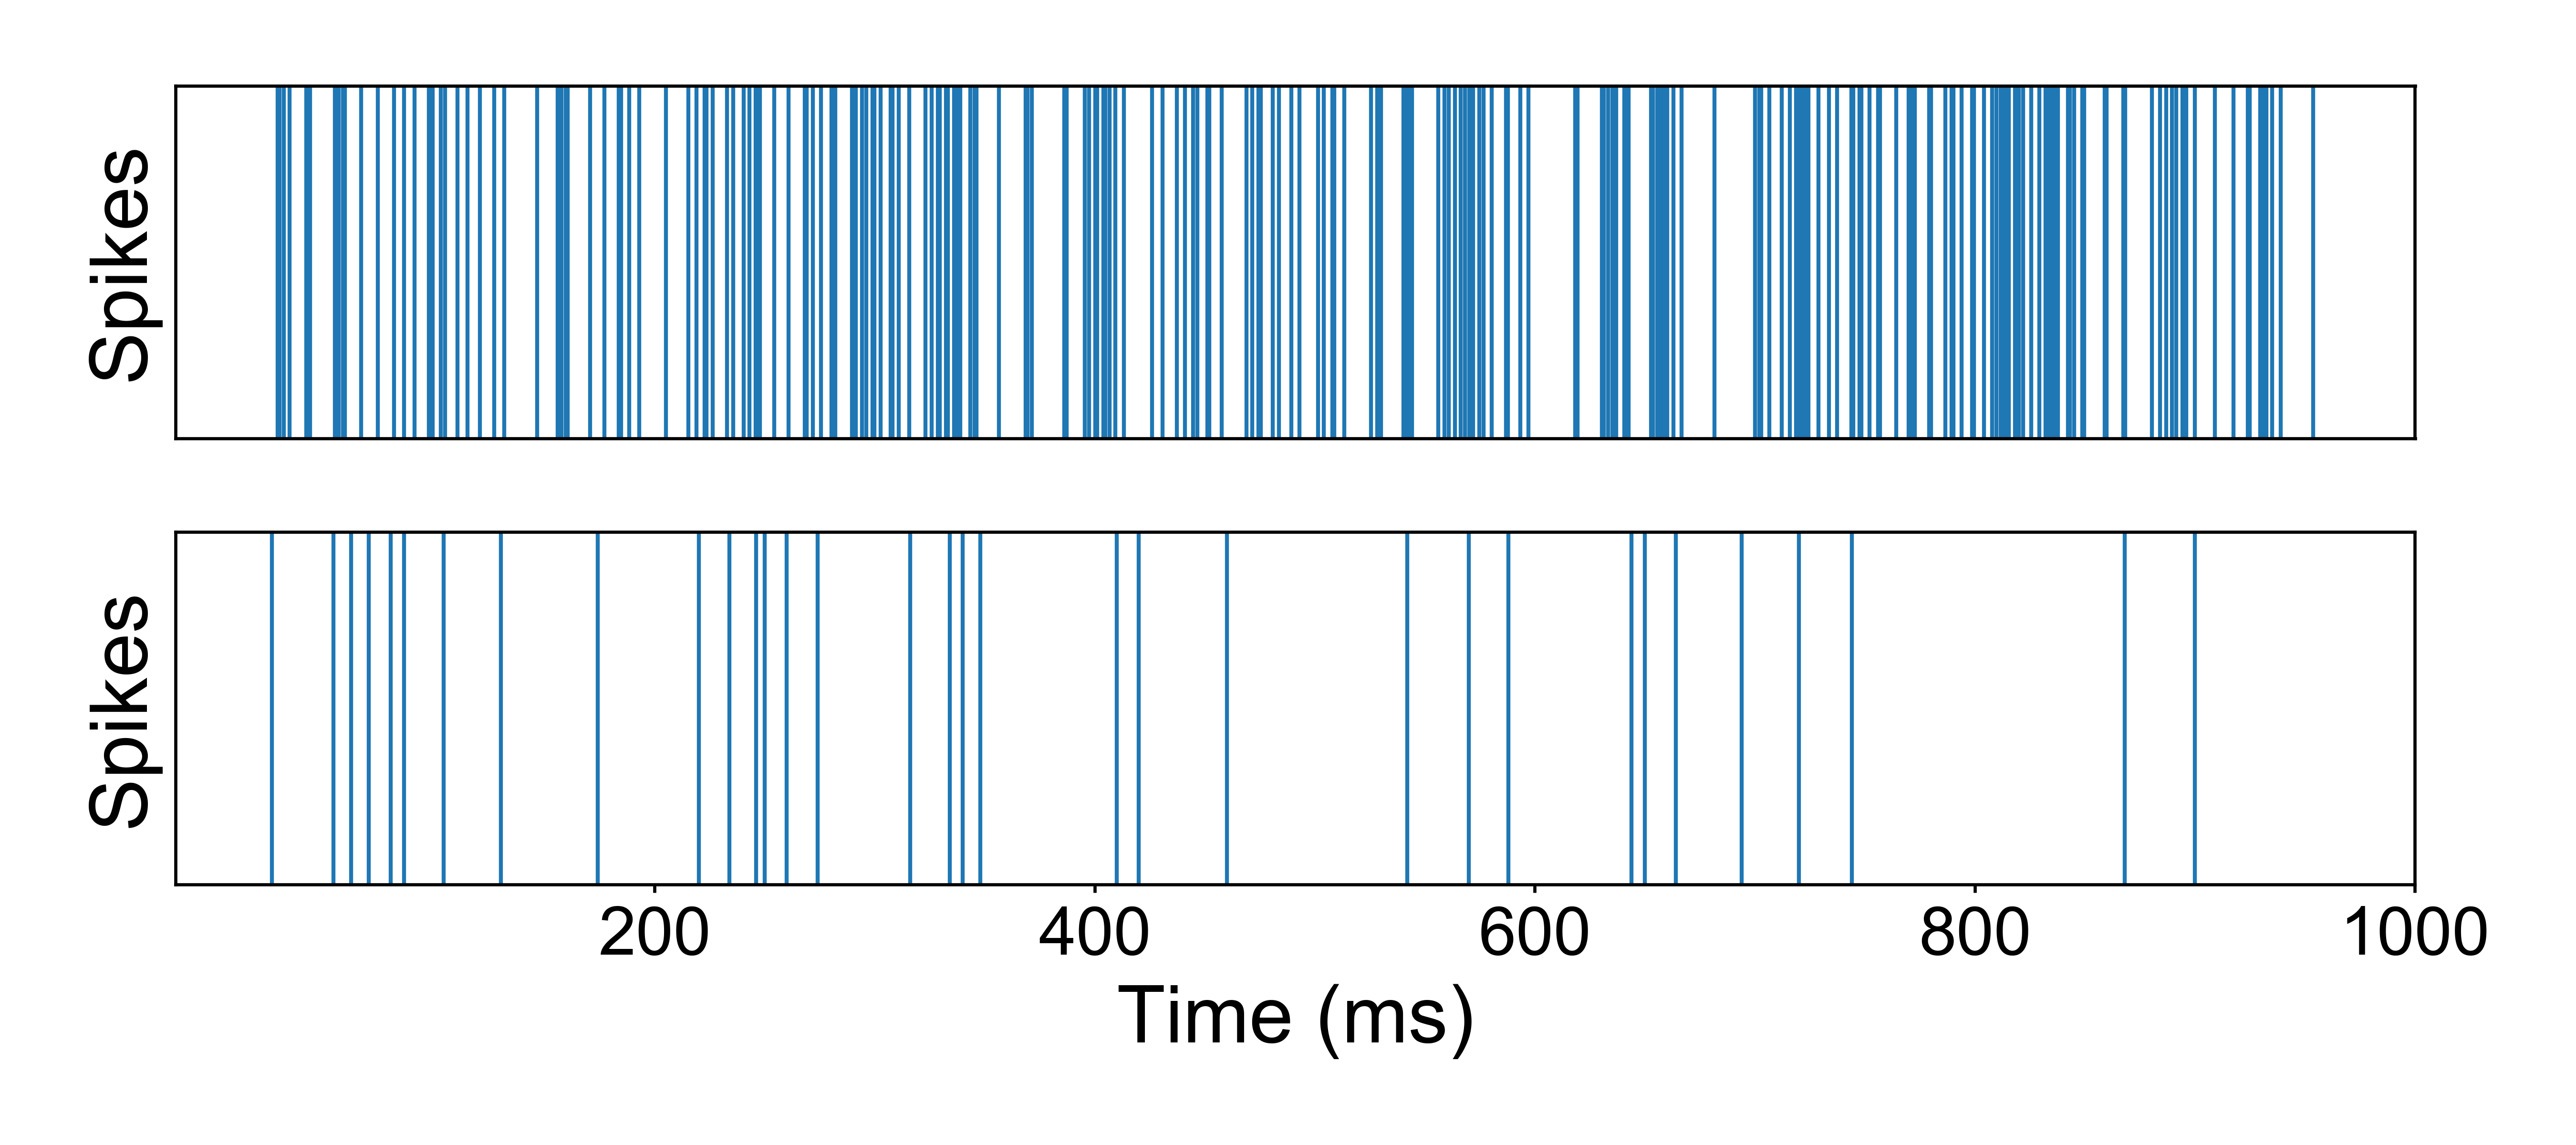
\includegraphics[width=.8\linewidth]{report3_fig14.png}
\caption[spt]{Up. Generating `spikes' with a probablity of $1/4$ 1000 times. Down. 1 second of simulated spiking activity, generated from a mean firing rate of 25 Hz, \textit{i.e.} there is $25/1000$ chance to have a spike at each ms.}\label{fig:fig1}
\end{figure}

The best way to make sense of spike trains is to look at the mean firing rate (\textit{i.e.} number of spike per second) in time. You can use such a number to simulate spiking activity (Figure \ref{fig:fig1} Down.) or you can use multiple recordings to compute an approximate firing rate. A convenient way to visualize multiple recording is through rasterplots: each row showing a spike train (Figure \ref{fig:fig2}). We can then compute the mean spike count or the firing rate in a given time period.

\begin{figure}[H]
\centering
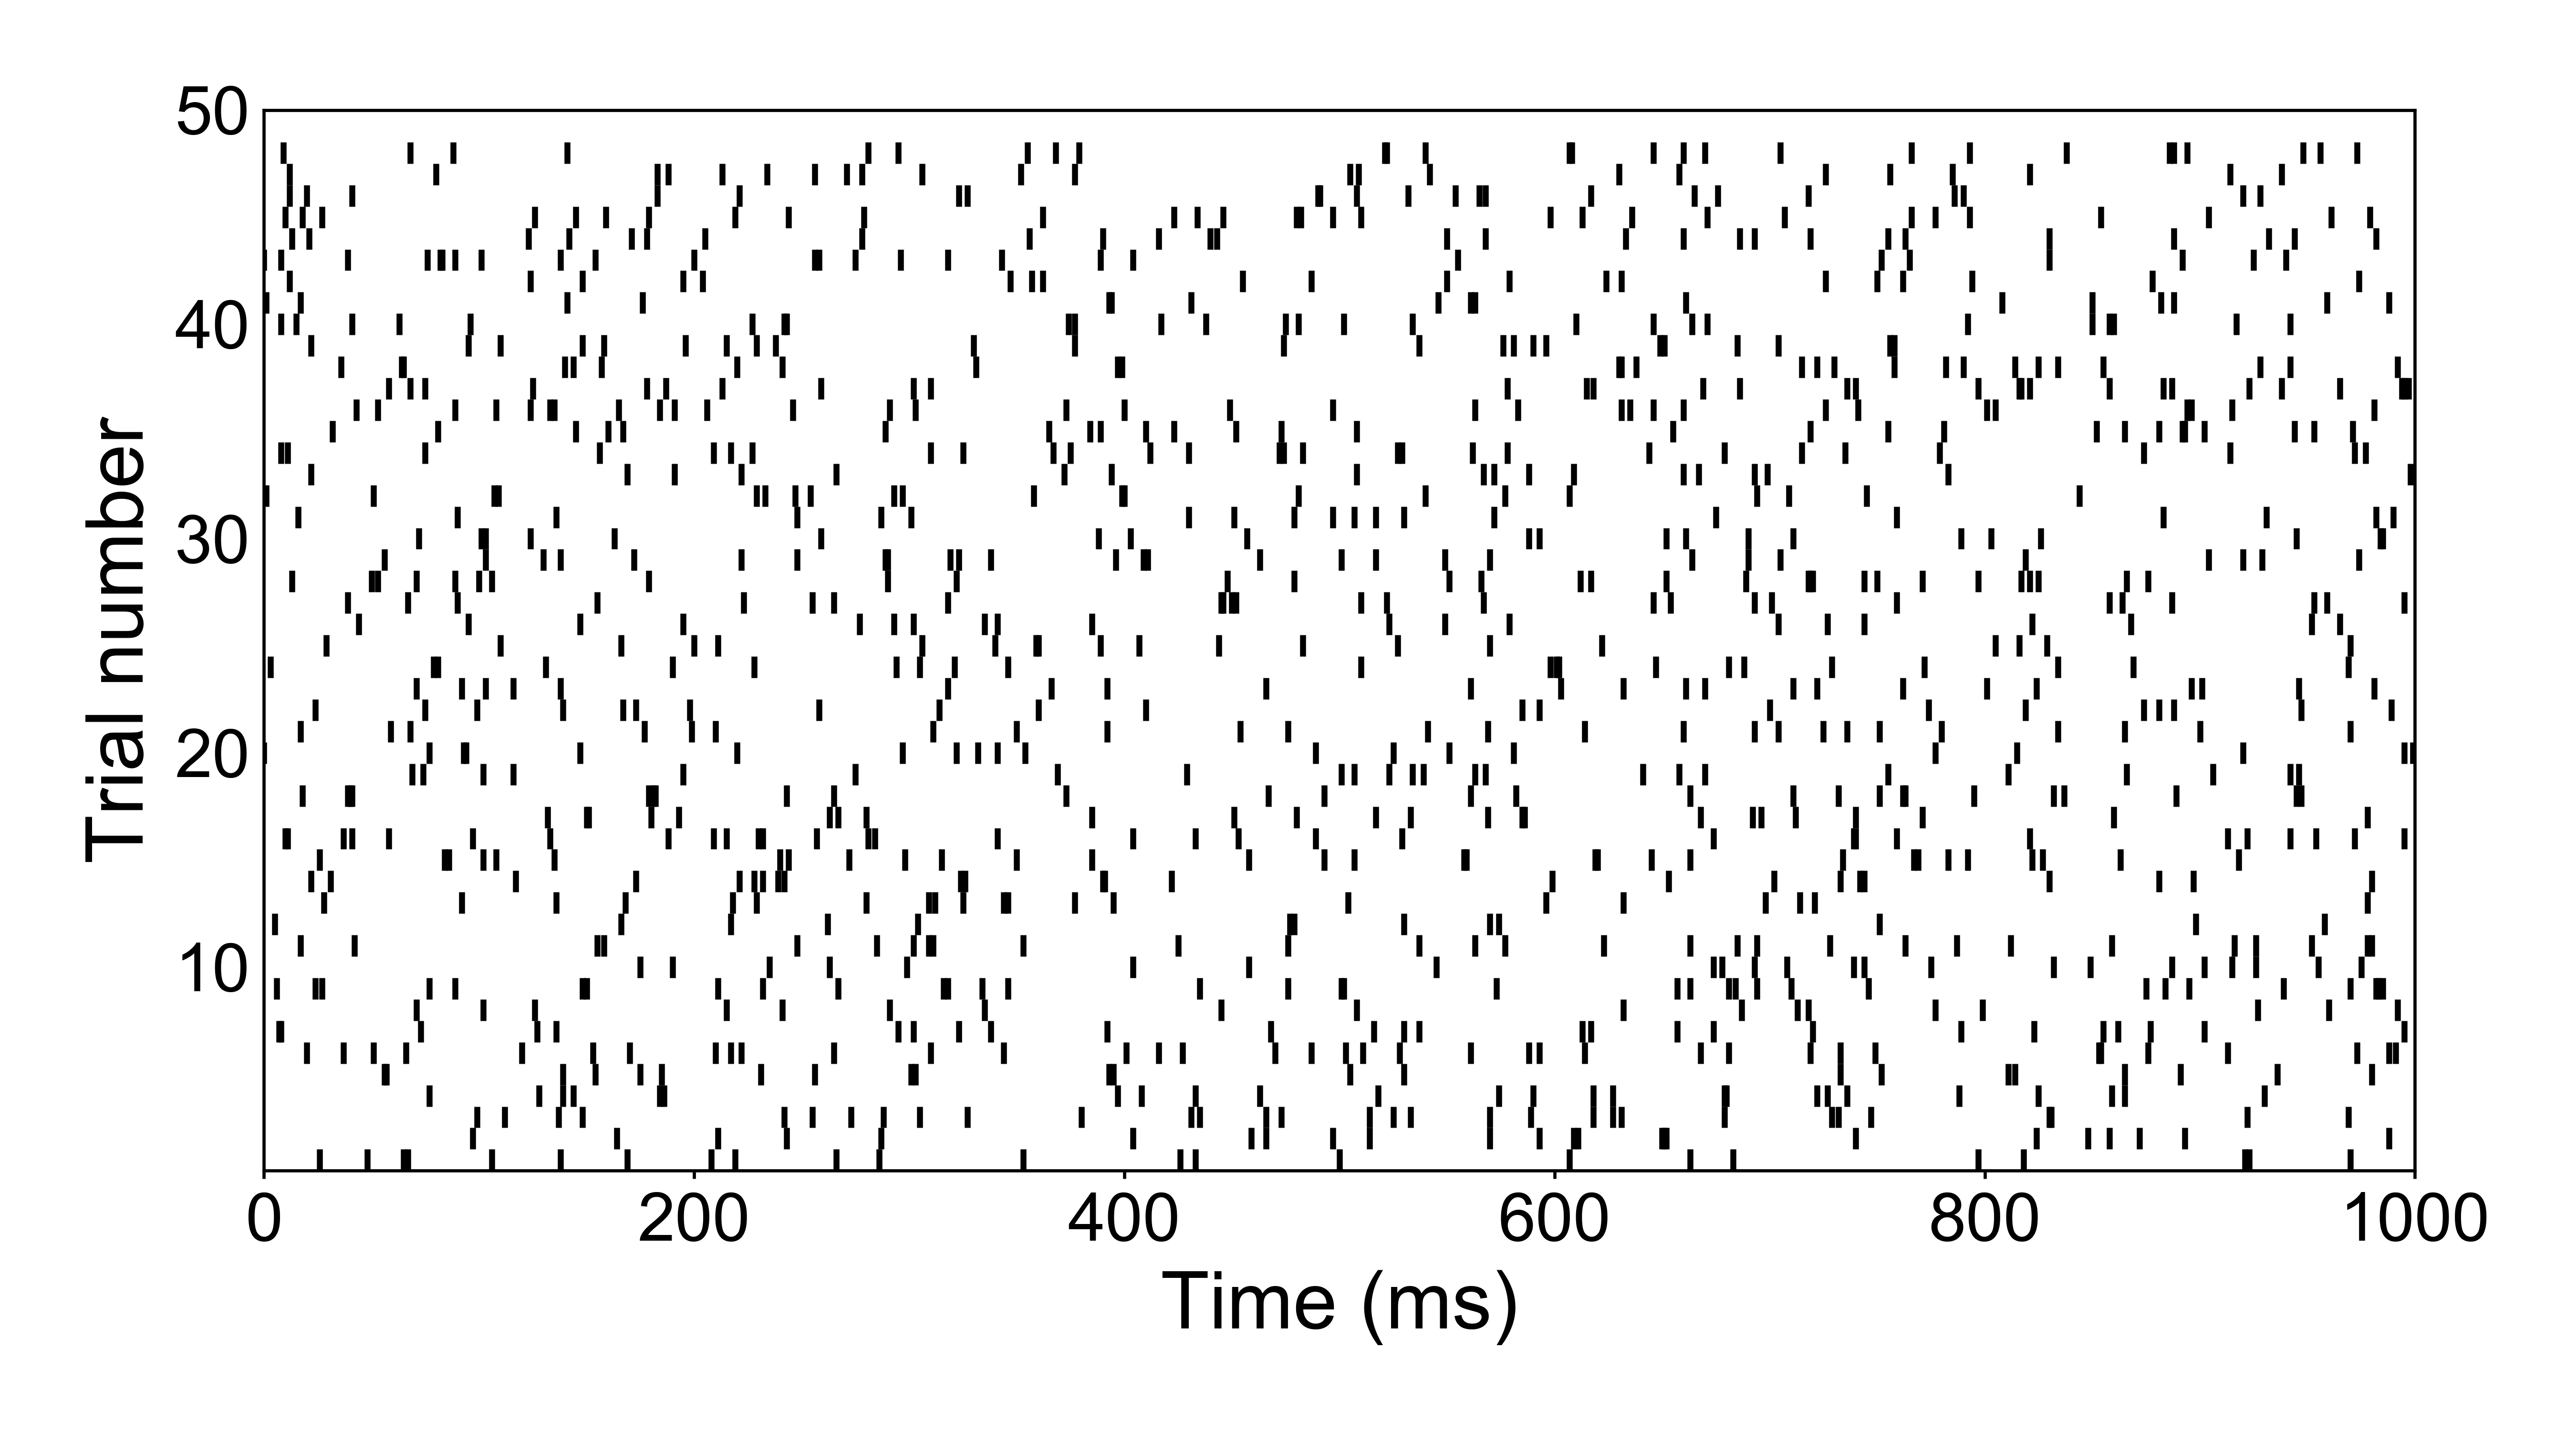
\includegraphics[width=.8\linewidth]{report3_fig3.png}
\caption[spt]{Rasterplot of 50 1s trials simulated with a firing rate of 25Hz.}\label{fig:fig2}
\end{figure}

Interestingly, because there is a high number of trials, the distribution of spike counts is almost normal (Figure \ref{fig:fig3} Left.). Moreover, the distribution of inter-spike intervals (ISI) shows an exponential decay, because, as the spike probability at each time point is independent, if you take a longer time period, the spike probability increases (Figure \ref{fig:fig3} Right.)

\begin{figure}[H]
\centering
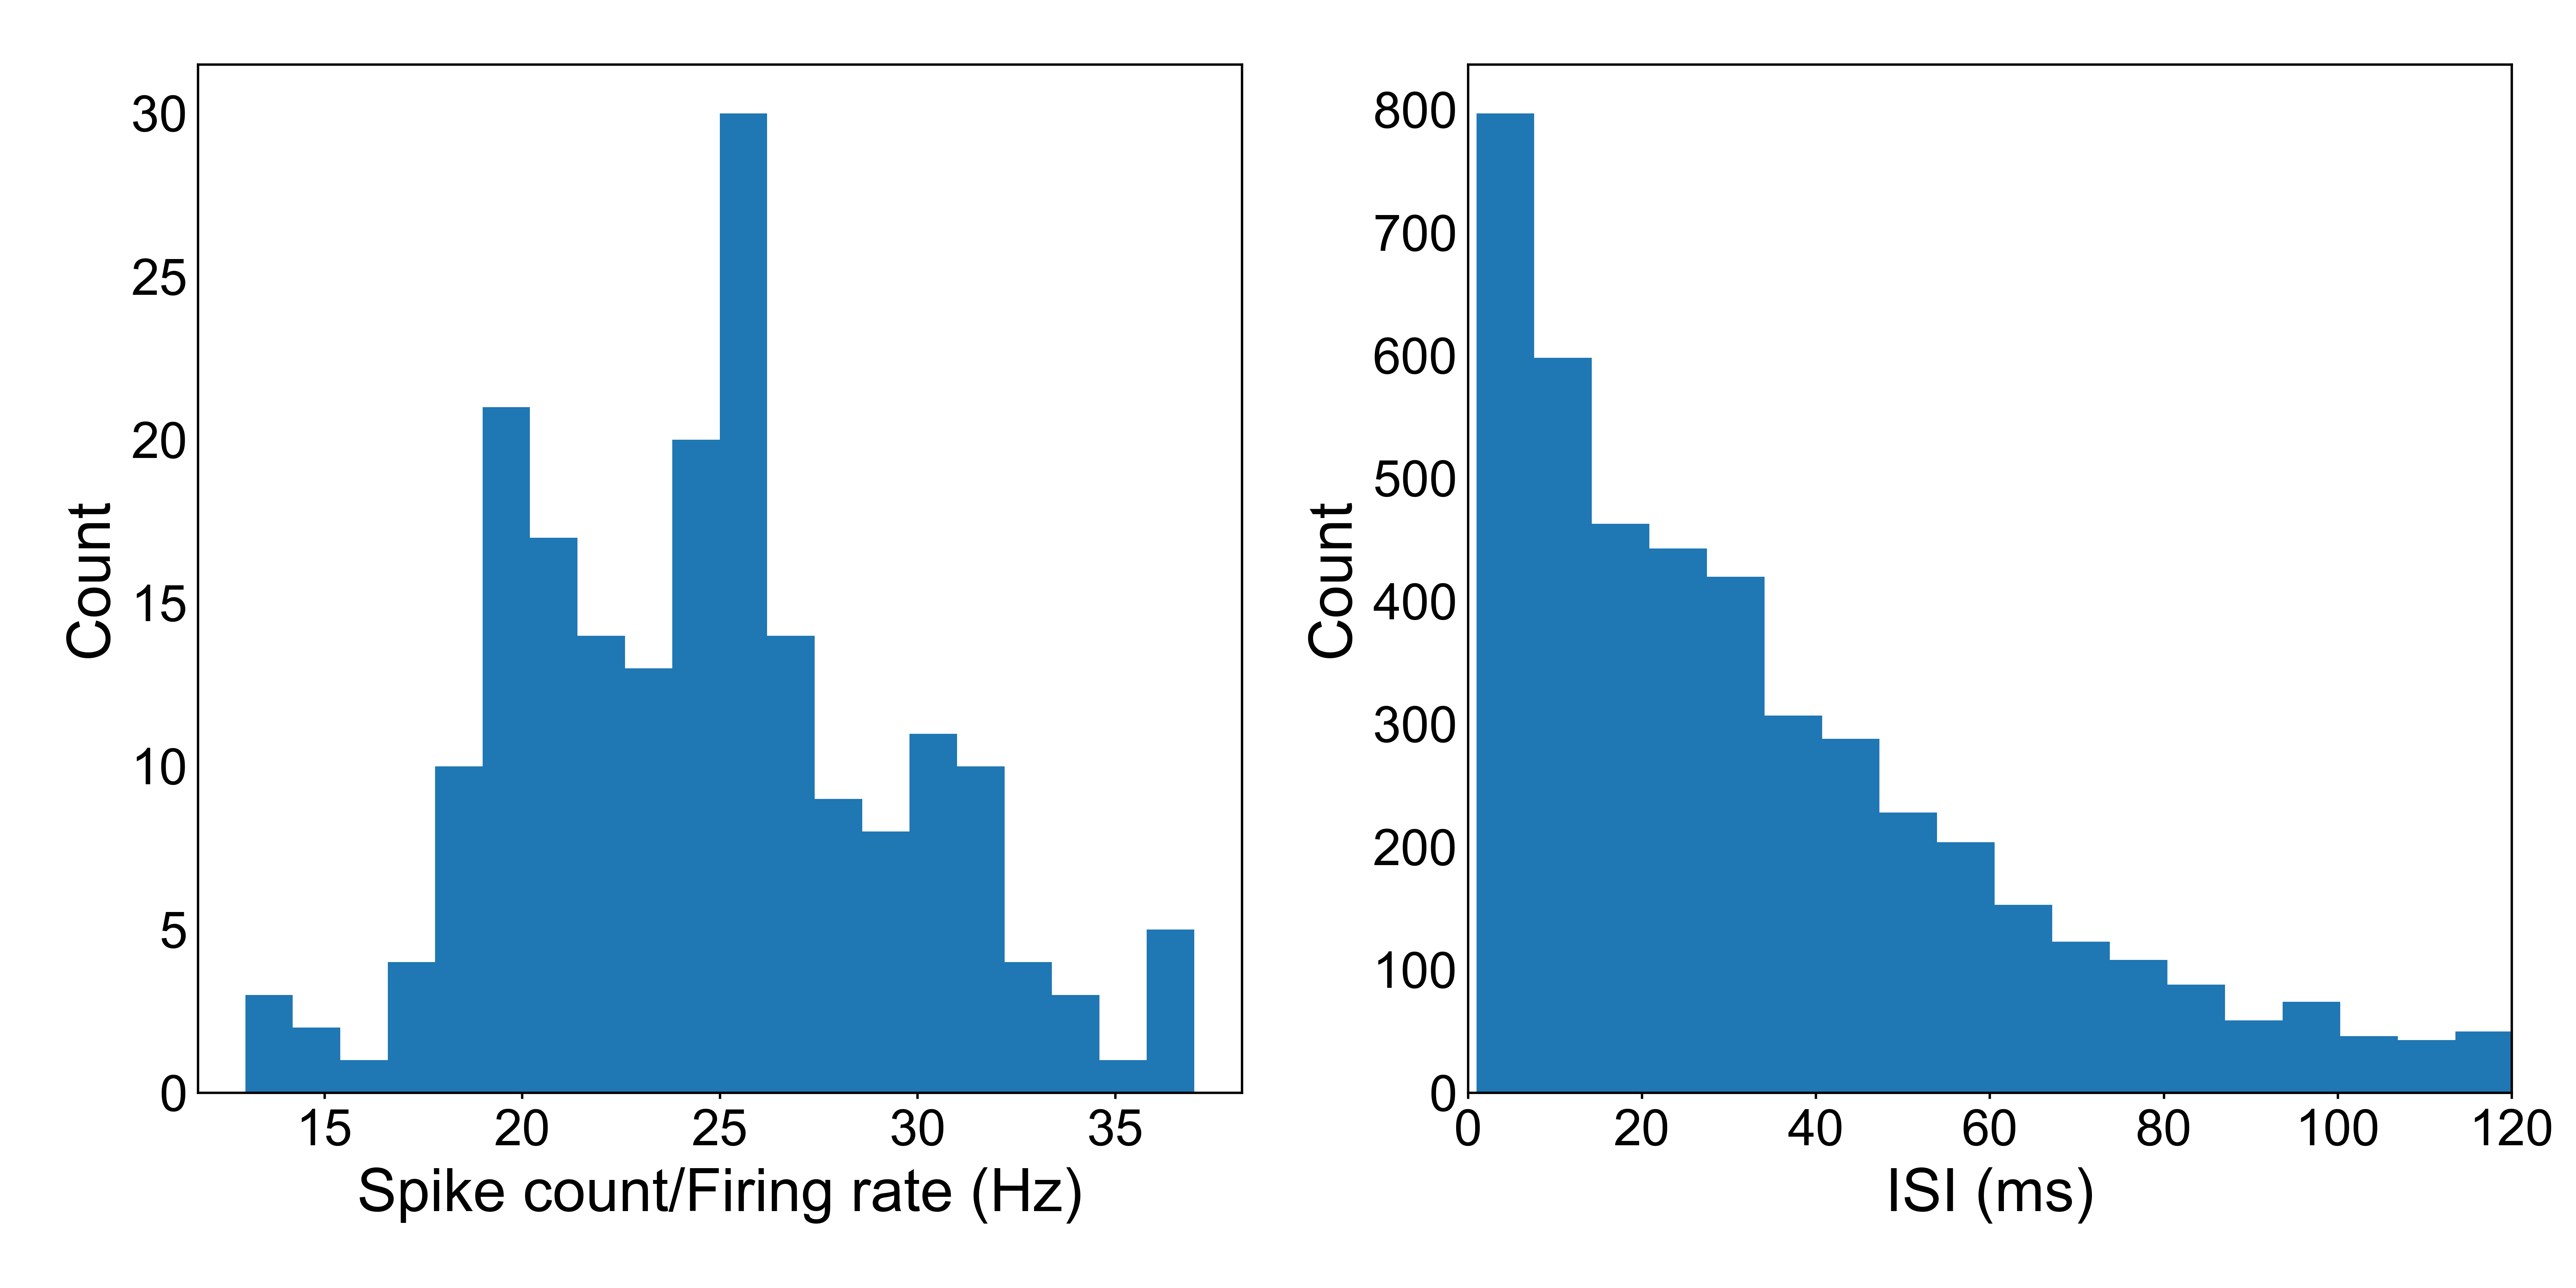
\includegraphics[width=.8\linewidth]{report3_fig15.png}
\caption[spt]{Left. Distribution of spike counts for 200 simulated spike trains with 25HZ. Right. Distribution of ISIs, disregarding the trial.}\label{fig:fig3}
\end{figure}
%----------------------------------------------------------------------------------------
%	SECTION 2
%----------------------------------------------------------------------------------------

\section{Analysis of spike trains}\label{ana}
\indent\indent Neuroscience experiments have shown that neurons have receptive fields (\textit{e.g.} a point in the visual field, a patch of skin, ...) for which they are reactive, \textit{i.e.} for which there firing rate increases, or even `encodes' the stimulus. For instance, figure \ref{fig:fig4} shows the spiking activity of a monkey's neuron in response to a 8.4Hz vibratory stimulation on the fingertips. The firing rate transliently every 120ms approximatly, \textit{i.e.} at a 8.4 Hz rate ($ 120 \times 8.4 \approx 1000$). Figure \ref{fig:fig5} shows recordings of the same neuron for different stimulation, always exhibiting the same pattern of imitation of the frequency. If one wants to infer a linear relationship between the firing rate and the frequency of stimulation - for instance to try to decode the spike activity recorded - one can see that in this case, the firing rate is approximatly 2.5 times the frequency of stimulation (Figure \ref{fig:fig6}. This seems rational given that there is approximatly 3 spikes every $1000/frequency$ ms.

\begin{figure}[H]
\centering
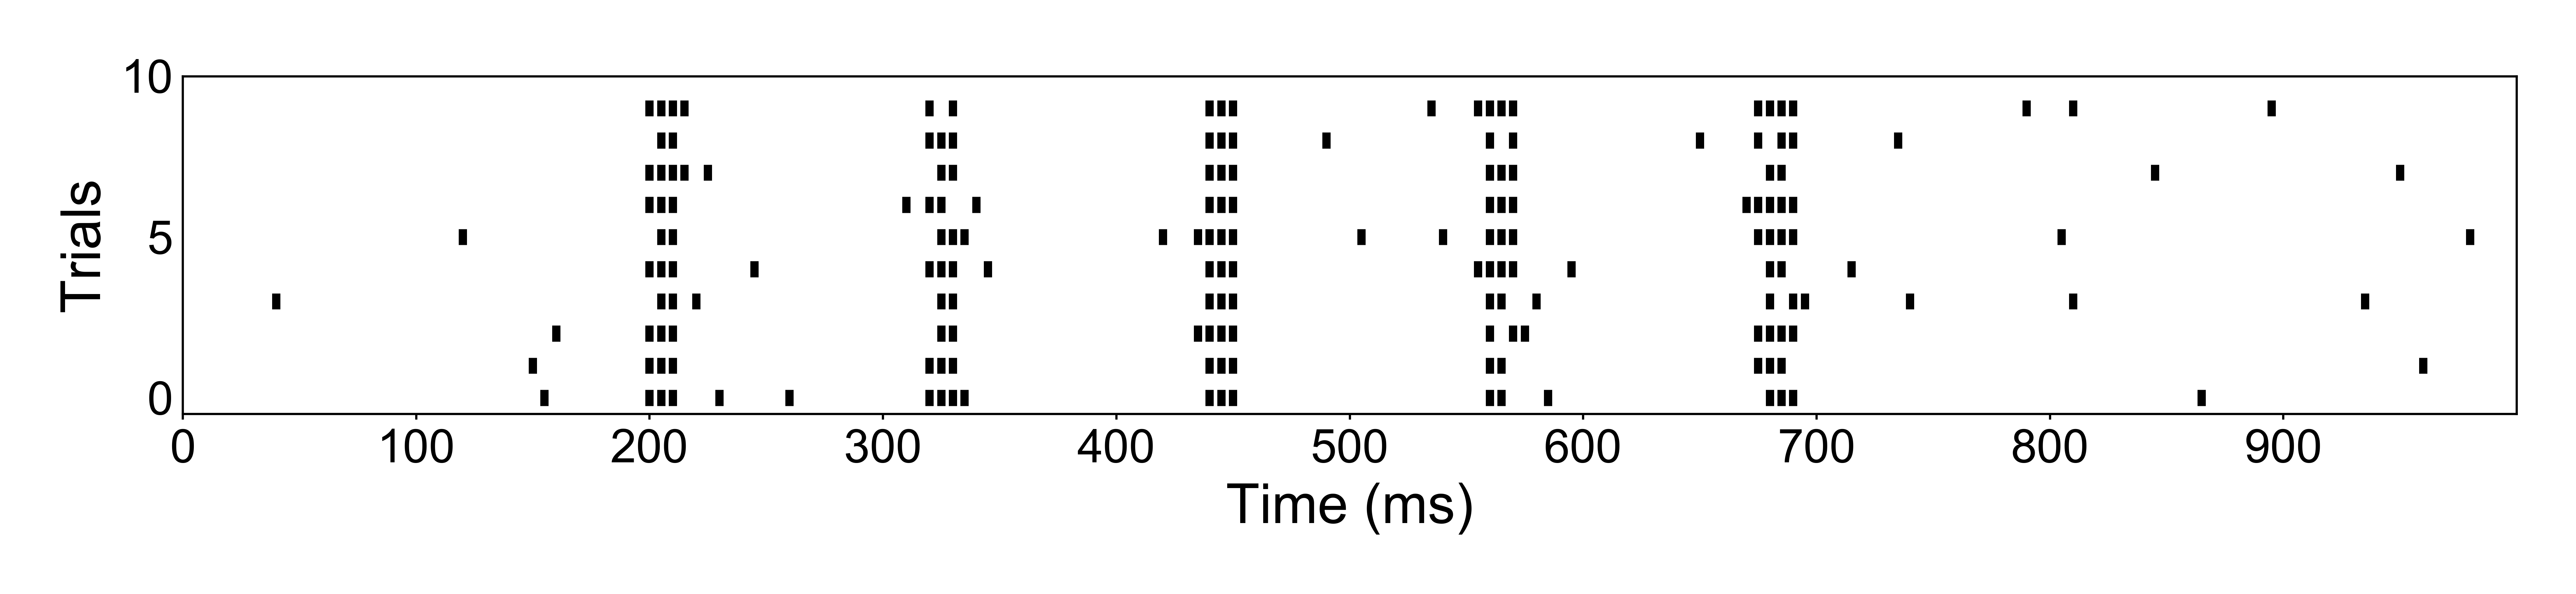
\includegraphics[width=.8\linewidth]{report3_fig6.png}
\caption[spt]{Spike trains emitted by a neuron in response to a vibratory stimulation (between 200 and 700ms).}\label{fig:fig4}
\end{figure}

\begin{figure}[H]
\centering
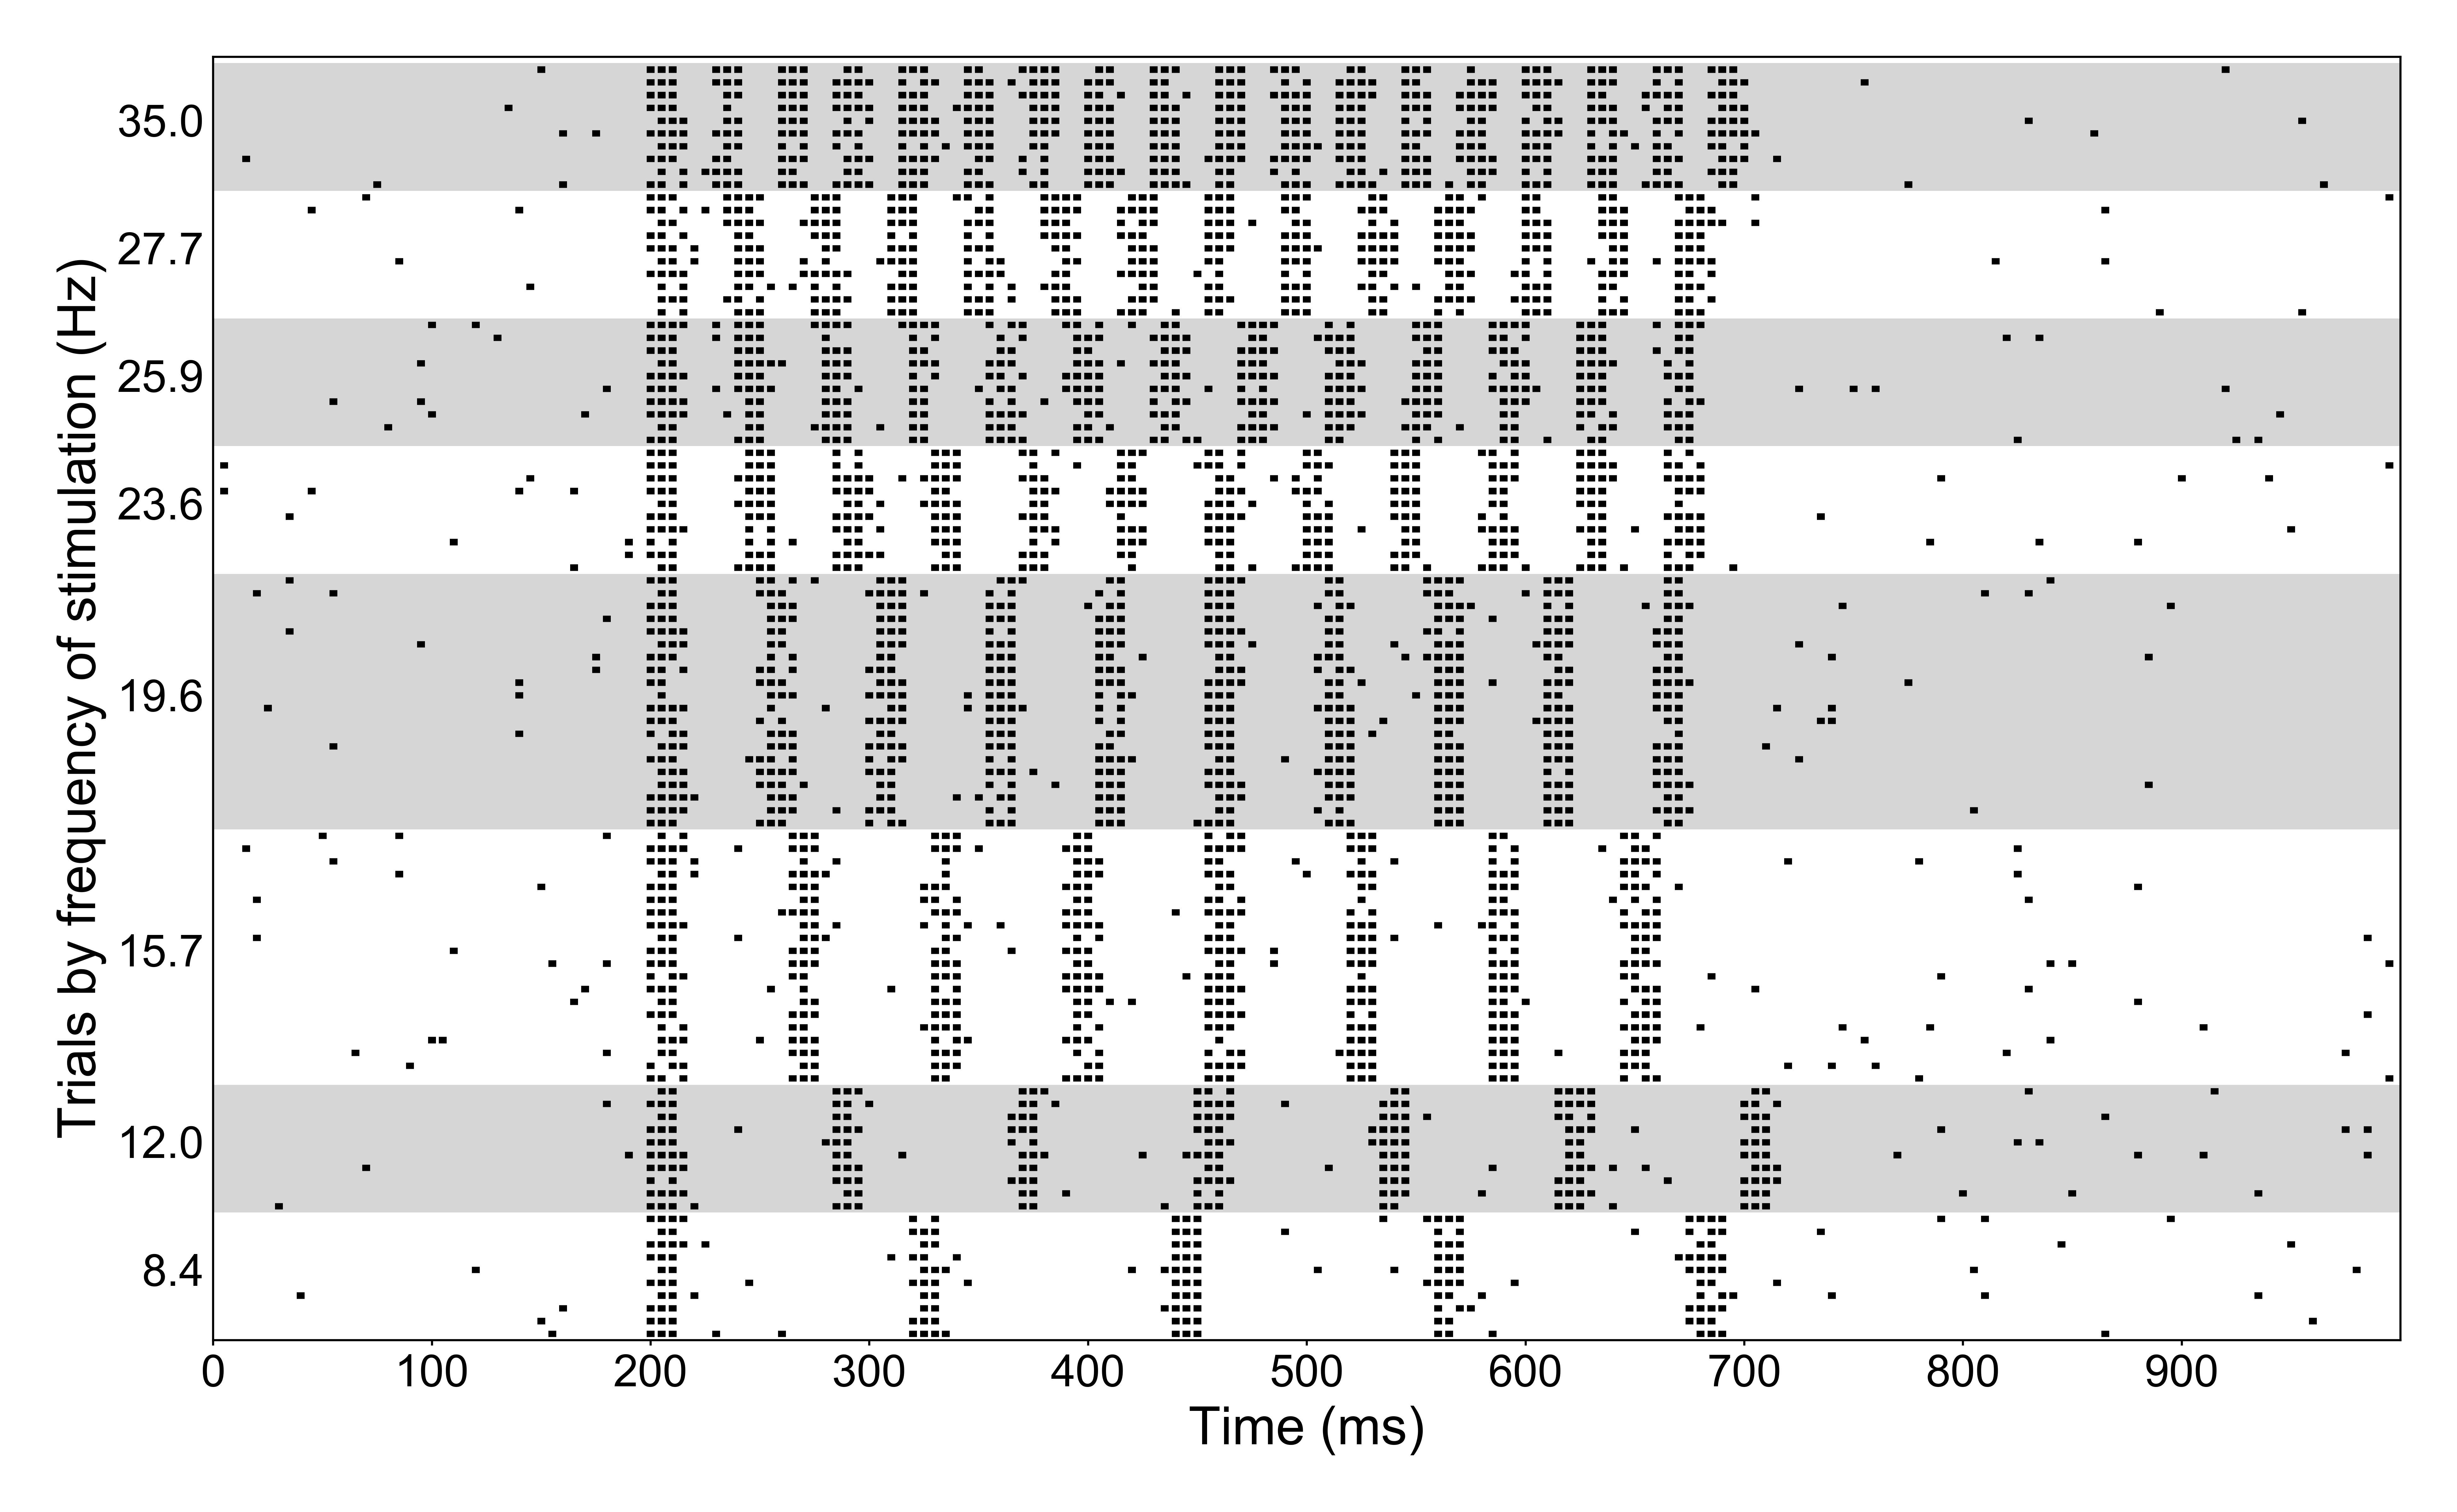
\includegraphics[width=1.1\linewidth]{report3_fig7.png}
\caption[spt]{Spike trains emitted by a neuron in response to different vibratory stimulation.}\label{fig:fig5}
\end{figure}

\begin{figure}[H]
\centering
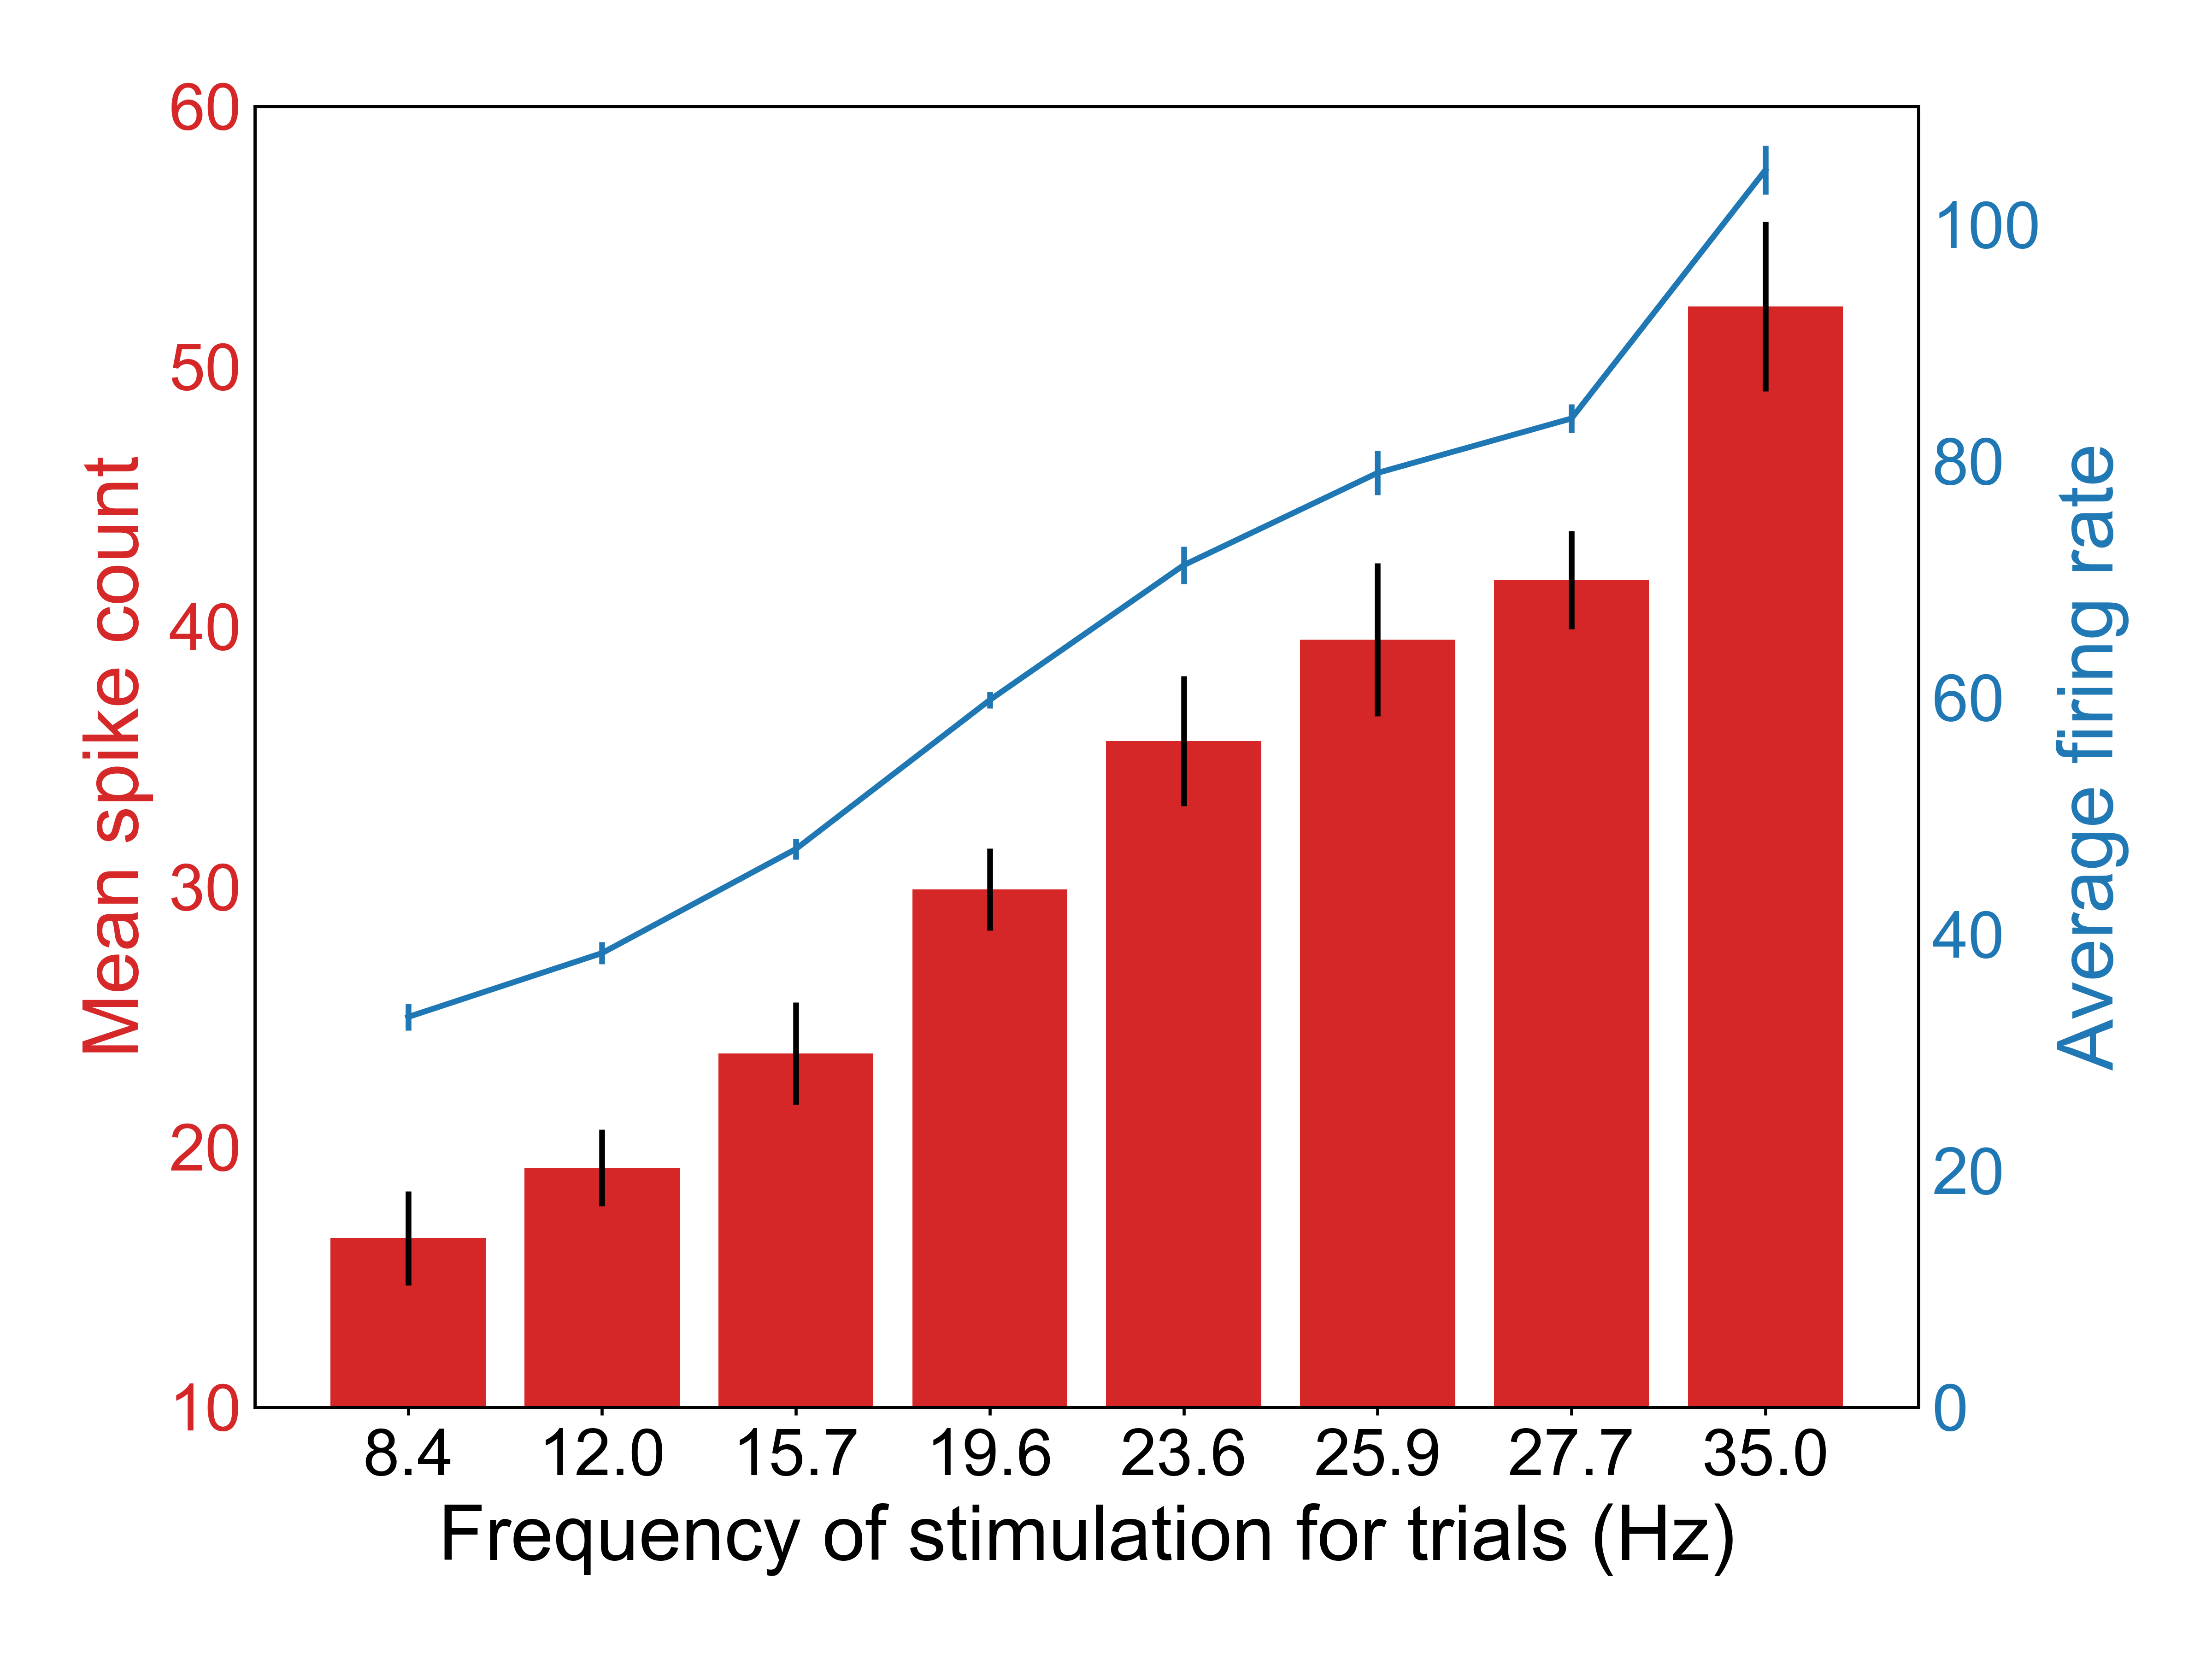
\includegraphics[width=.8\linewidth]{report3_fig8.png}
\caption[spt]{Spike count (error bars show standard deviation) and firing rate (standard error of the mean) of neuron during stimulation periods, for each frequency of stimulation. }\label{fig:fig6}
\end{figure}


%----------------------------------------------------------------------------------------
%	SECTION 3
%----------------------------------------------------------------------------------------

\section{Integrate-and-fire neurons}\label{int}
It is possible to approximate a neuron's membrane behavior with the following equation,  called the Leaky Integrate and Fire model (LIF):


\begin{align*}
  C\frac{dV(t)}{dt} = g_L(E_L - V(t)) + I
\end{align*}
\noindent where $C$ is the membrane capacitance, $g_L$ its conductance and $E_L$ its equilibrium potential. All those parameters are measurable experimentally.

\indent This differential equation can be solved numerically using Euler's method:
\begin{align*}
  V(t+\Delta t) &= V(t) + \frac{dV(t)}{dt} \Delta t\\
                &= V(t) + \frac{1}{C} \; \big( g_L(E_L - V(t)) + I \big)
\end{align*}


Let, for simplicity, $C= 1$ nF, $E_L=-70$ mV (the most usual equilibrium) and $g_L=0.1$ µS. To solve it we can say that $V(0)=E_L$ and see how the system evolves for different current injected. Figure \ref{fig:fig7} shows that the membrane potential $V(t)$ shows exponential convergence towards a certain potential, depending on the input current.
\begin{figure}[H]
\centering
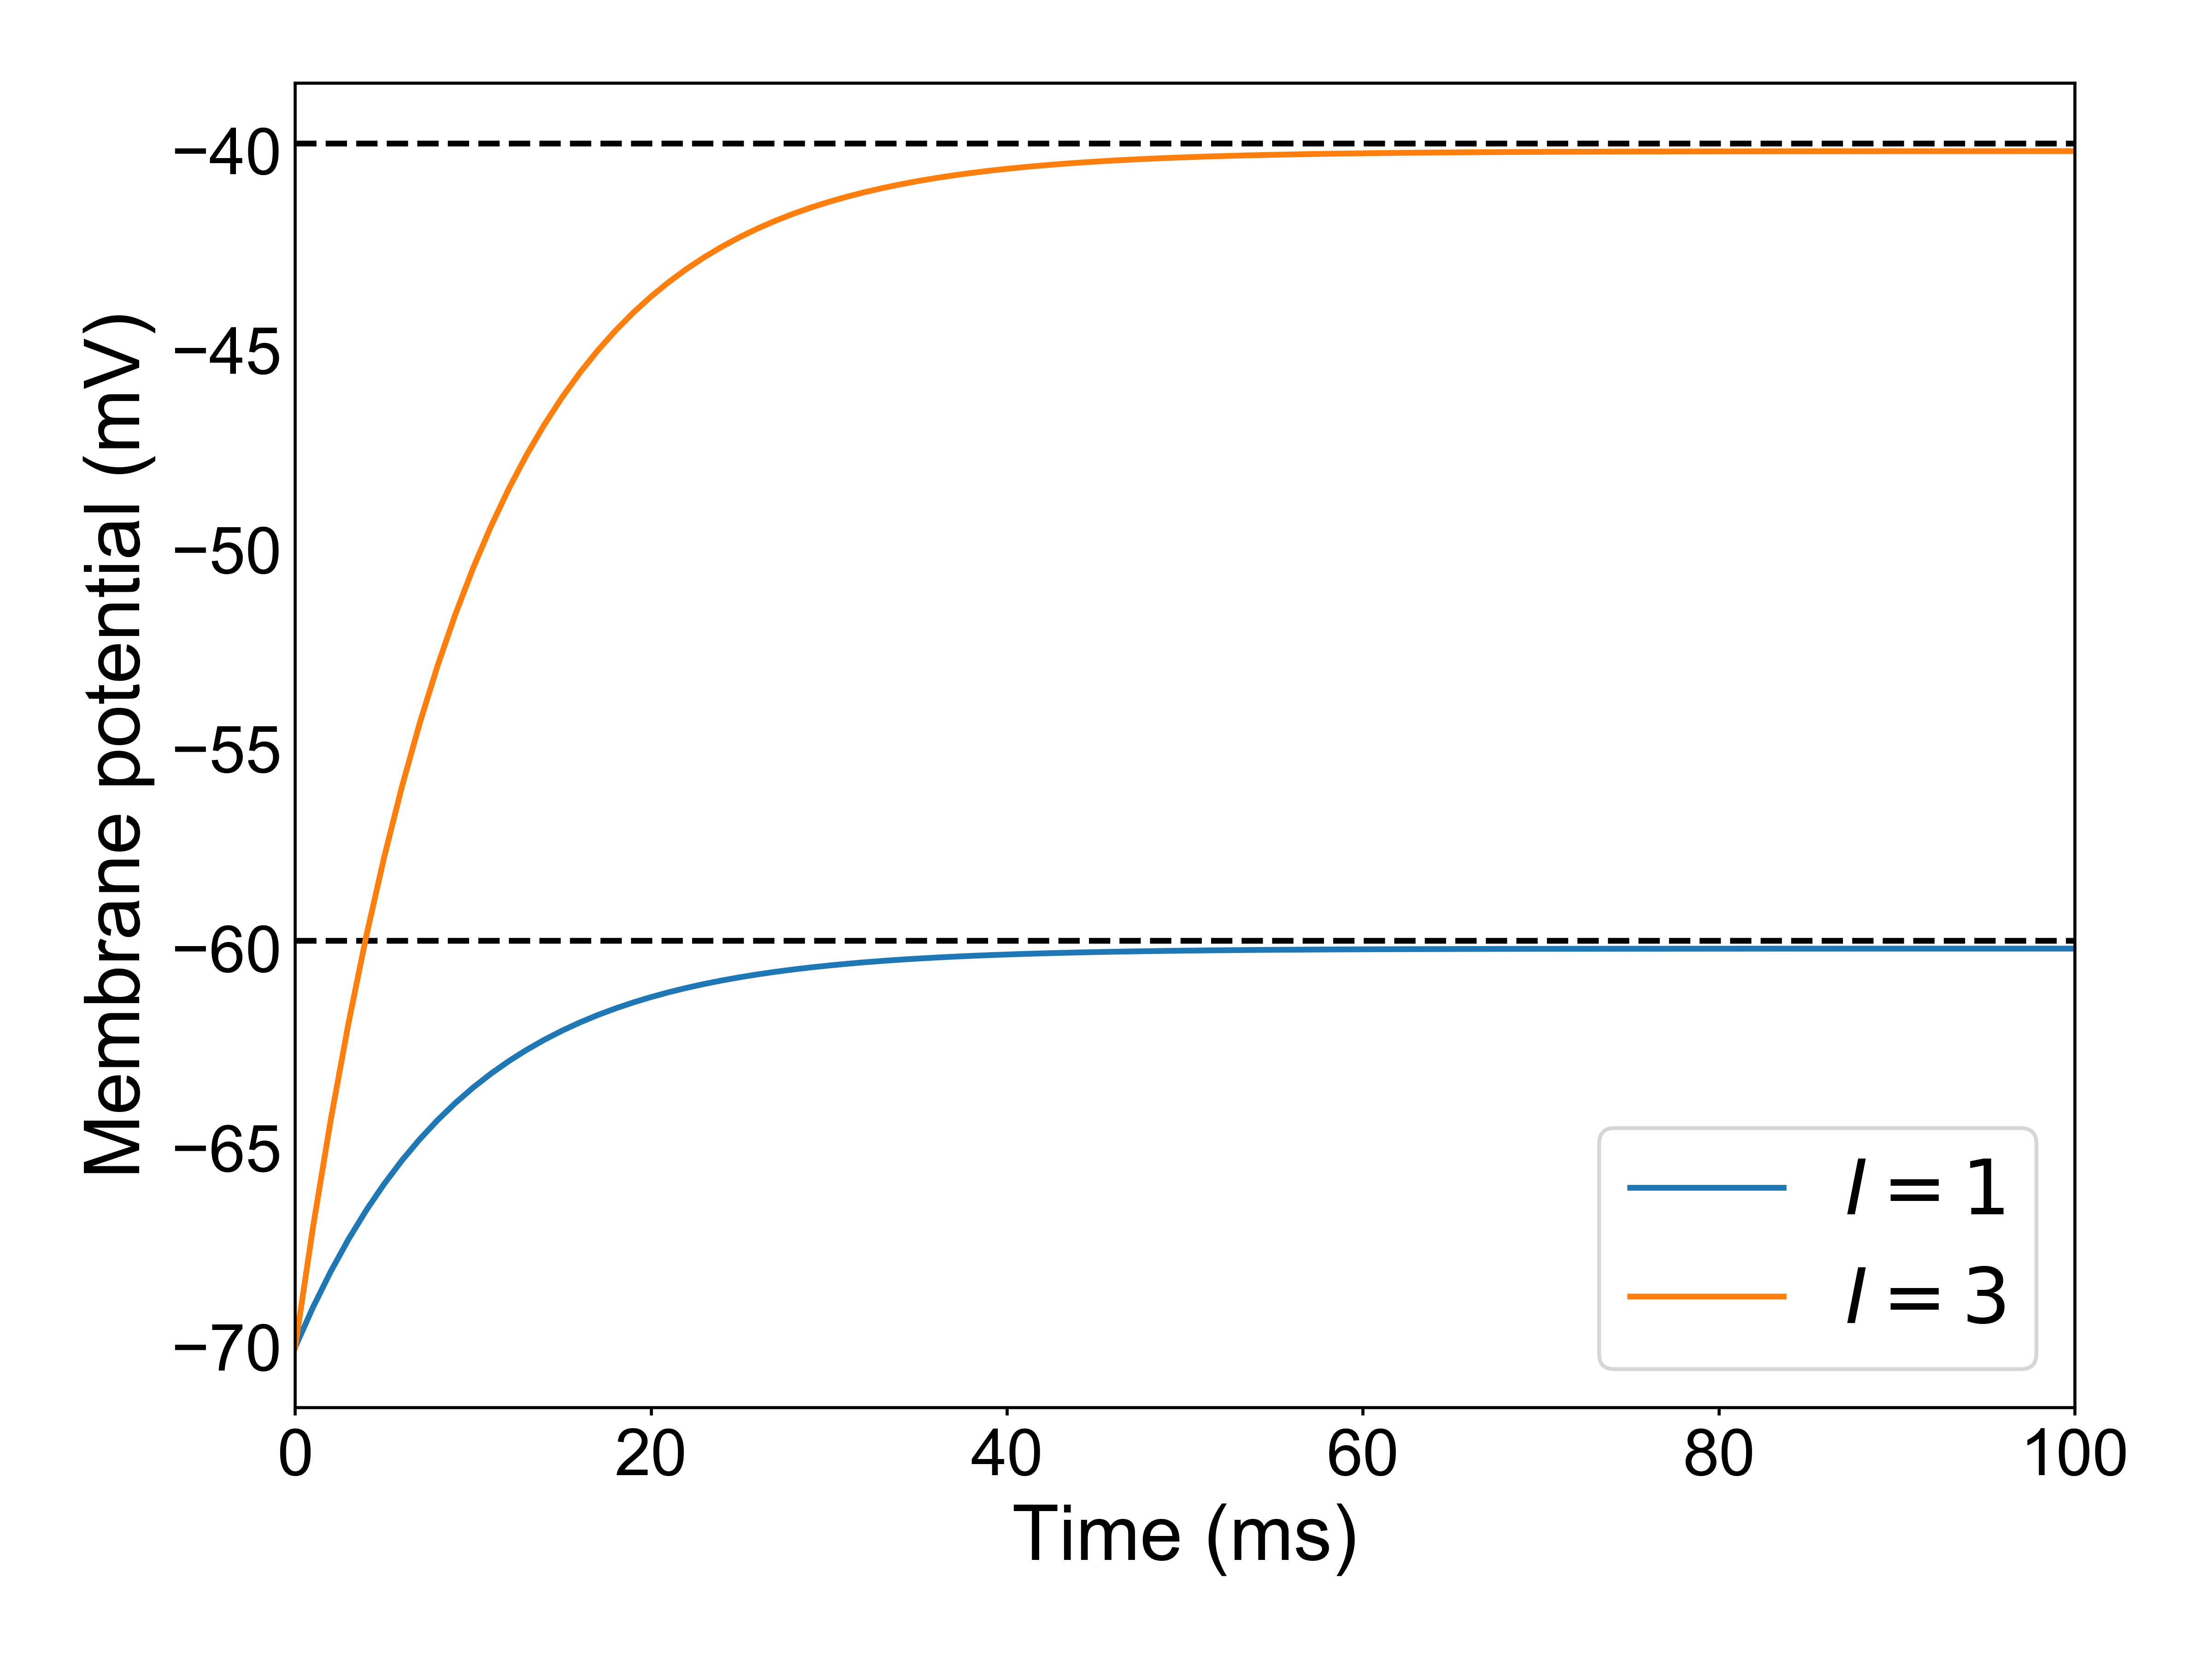
\includegraphics[width=.8\linewidth]{report3_fig9.png}
\caption[growing population]{Membrane potential V(t) in time for different injected currents.}\label{fig:fig7}
\end{figure}

As we can see, this model doesn't account for the spiking behavior of neurons, but we can artificially add it, by recording a spike when $V(t)$ reaches a threshold $V_{th}$ (for instance -63mV) and immediatly `resetting' $V(t)$ to a given potential $V_r$, for instance $E_L$. We can also artificially add the refractory period (RP) of neurons, which is a measurable time period after a spike, for which it isn't able to generate a new spike, because of some biophysical properties of the channels (Figure \ref{fig:fig8}).

\begin{figure}[H]
\centering
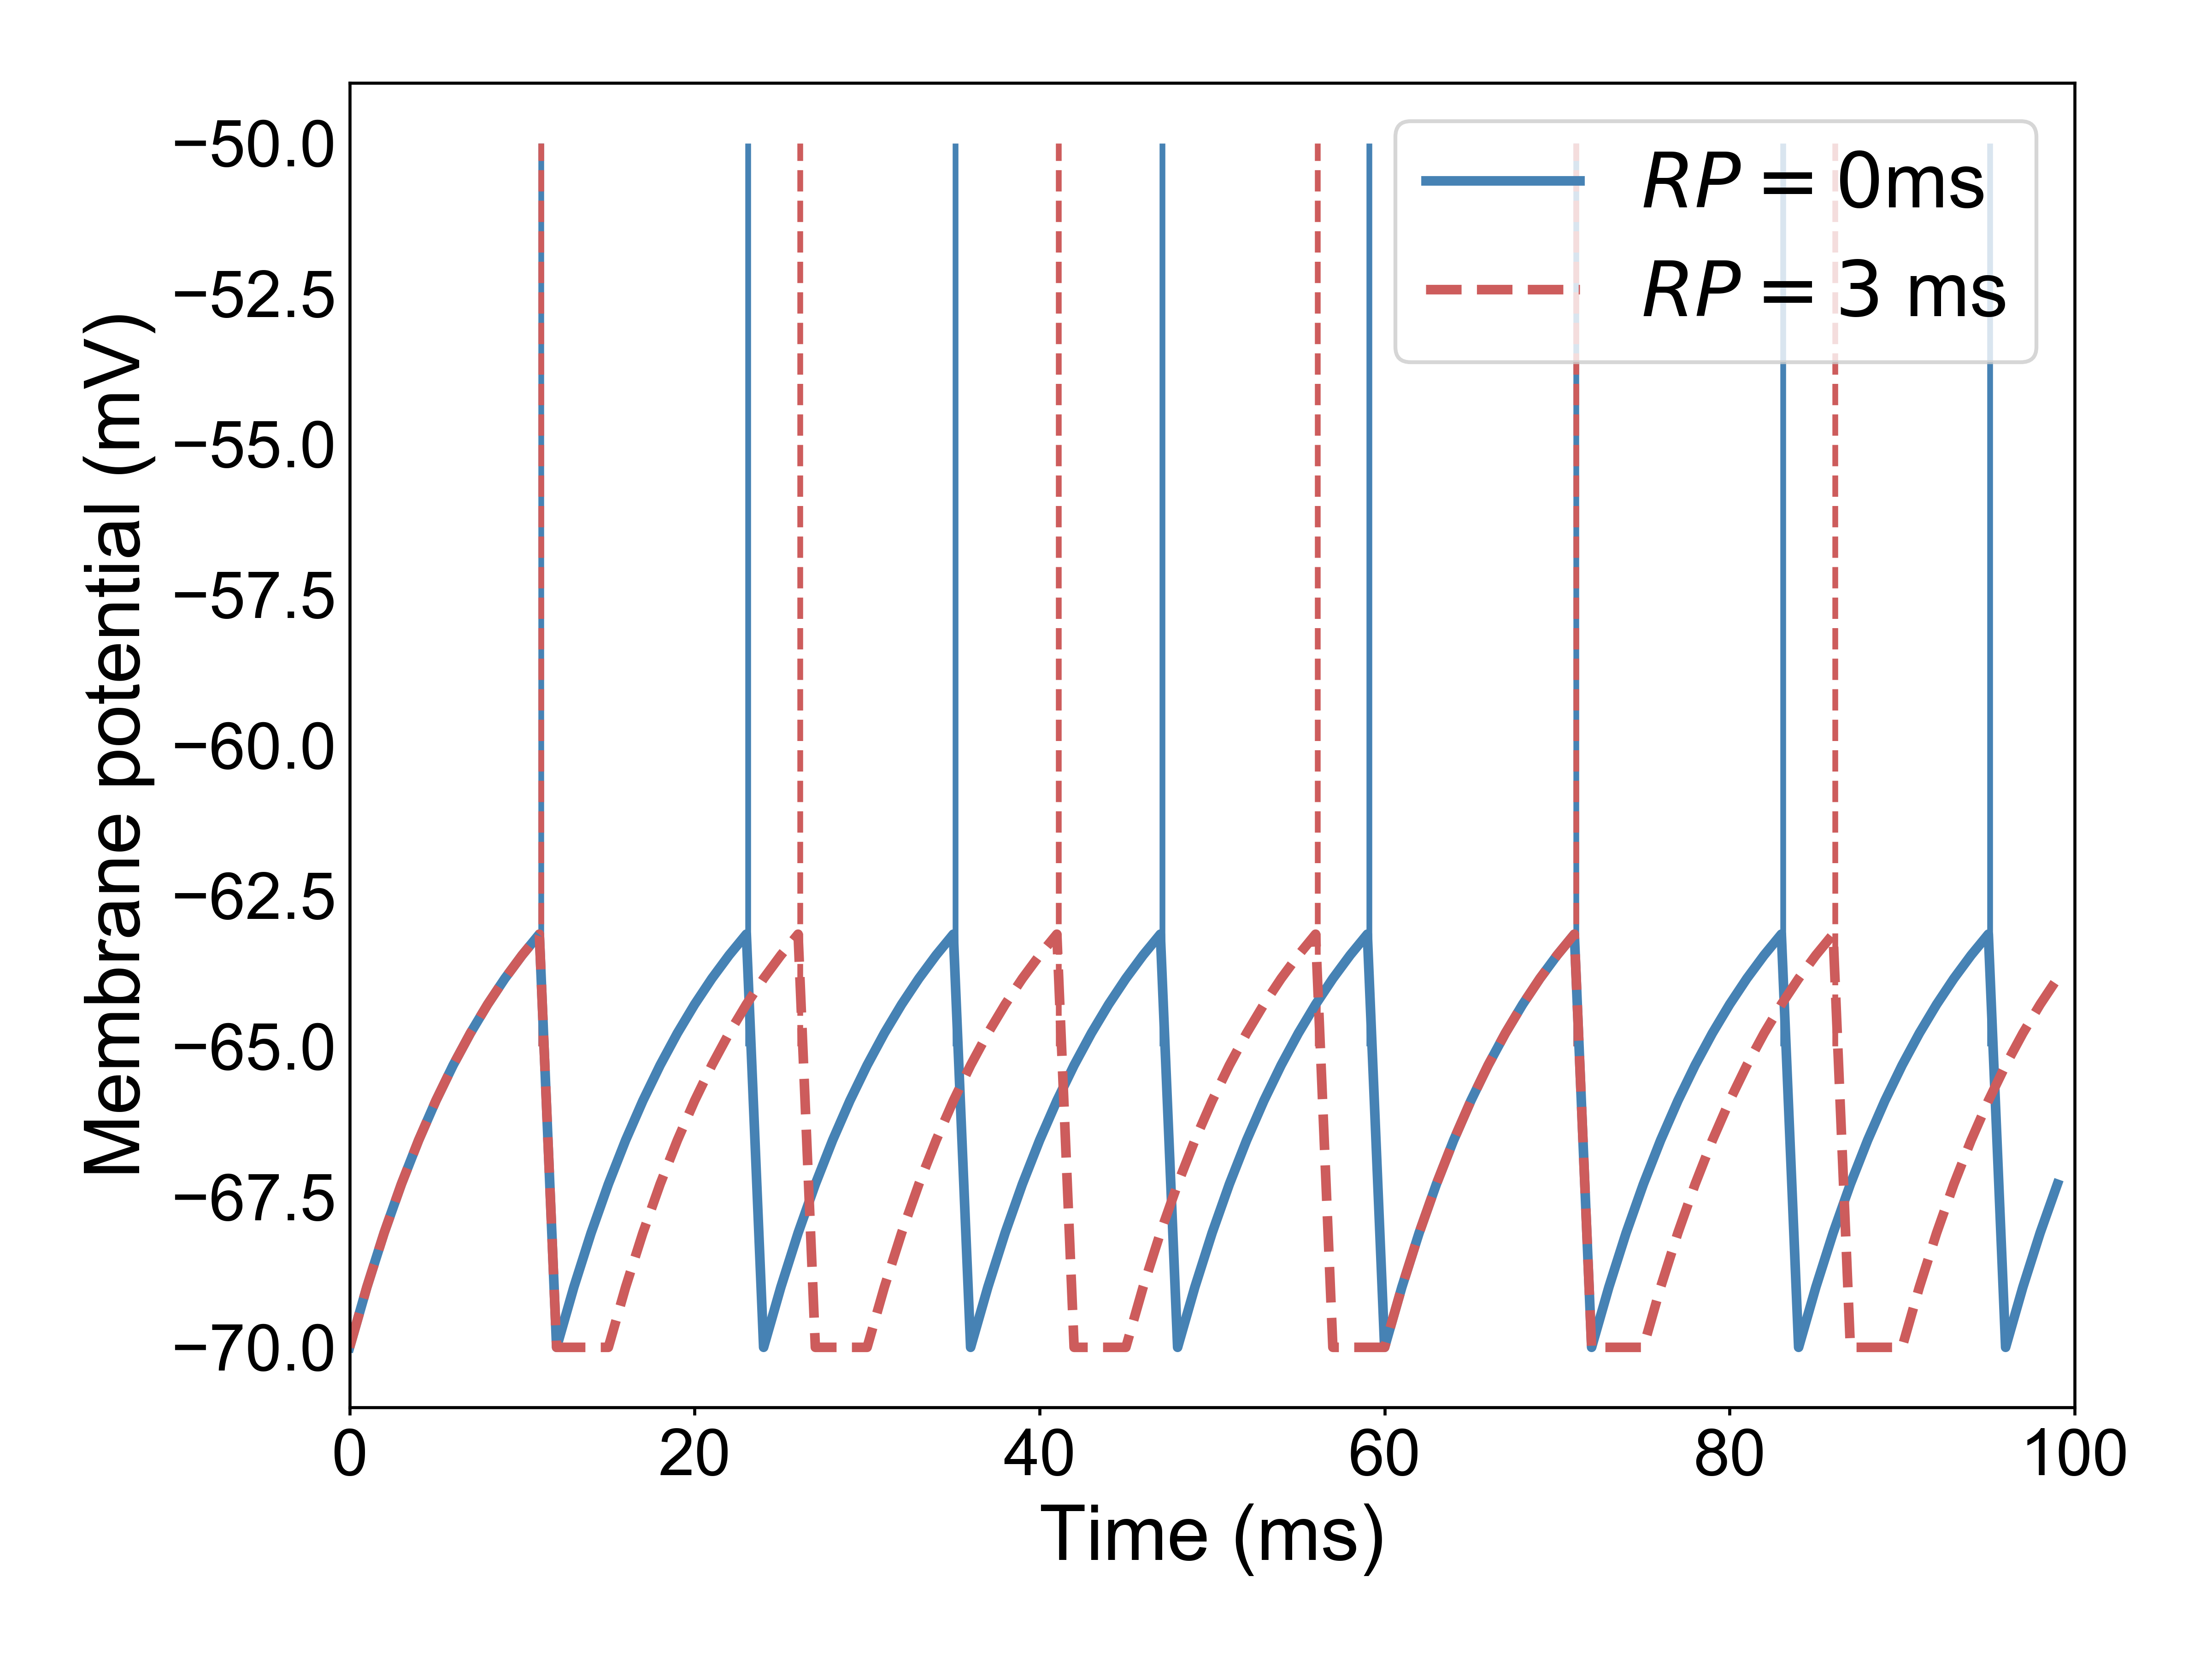
\includegraphics[width=.8\linewidth]{report3_fig11.png}
\caption[growing population]{Membrane potential V(t) in time, with an injected current $I=1$, with a reset mechanism added, and different RPs.}\label{fig:fig8}
\end{figure}

To continue to make the neuronal membrane dynamics more realistic, one can add a white noise term $\eta(t)$ (number from a gaussian distribution of mean 0 and standard deviation 1) in the equation, where $\sigma$ determines the magnitude of the noise:
\begin{align*}
  C\frac{dV(t)}{dt} = g_L(E_L - V(t)) + I + \sigma\eta(t)
\end{align*}
So,
\begin{align*}
  V(t+\Delta t) &= V(t) + \frac{dV(t)}{dt} \Delta t + \sigma\eta(t)\sqrt{\Delta t}\\
                &= V(t) + g_L(E_L - V(t)) + I + \sigma\eta(t)
\end{align*}

\noindent as $\Delta t = 1$ms and $C=1$.\\

Figure \ref{fig:fig9} shows that the spiking rate is only slightly irregular with a little noise, but becomes rapidly erratic as the noise increases.

\begin{figure}[H]
\centering
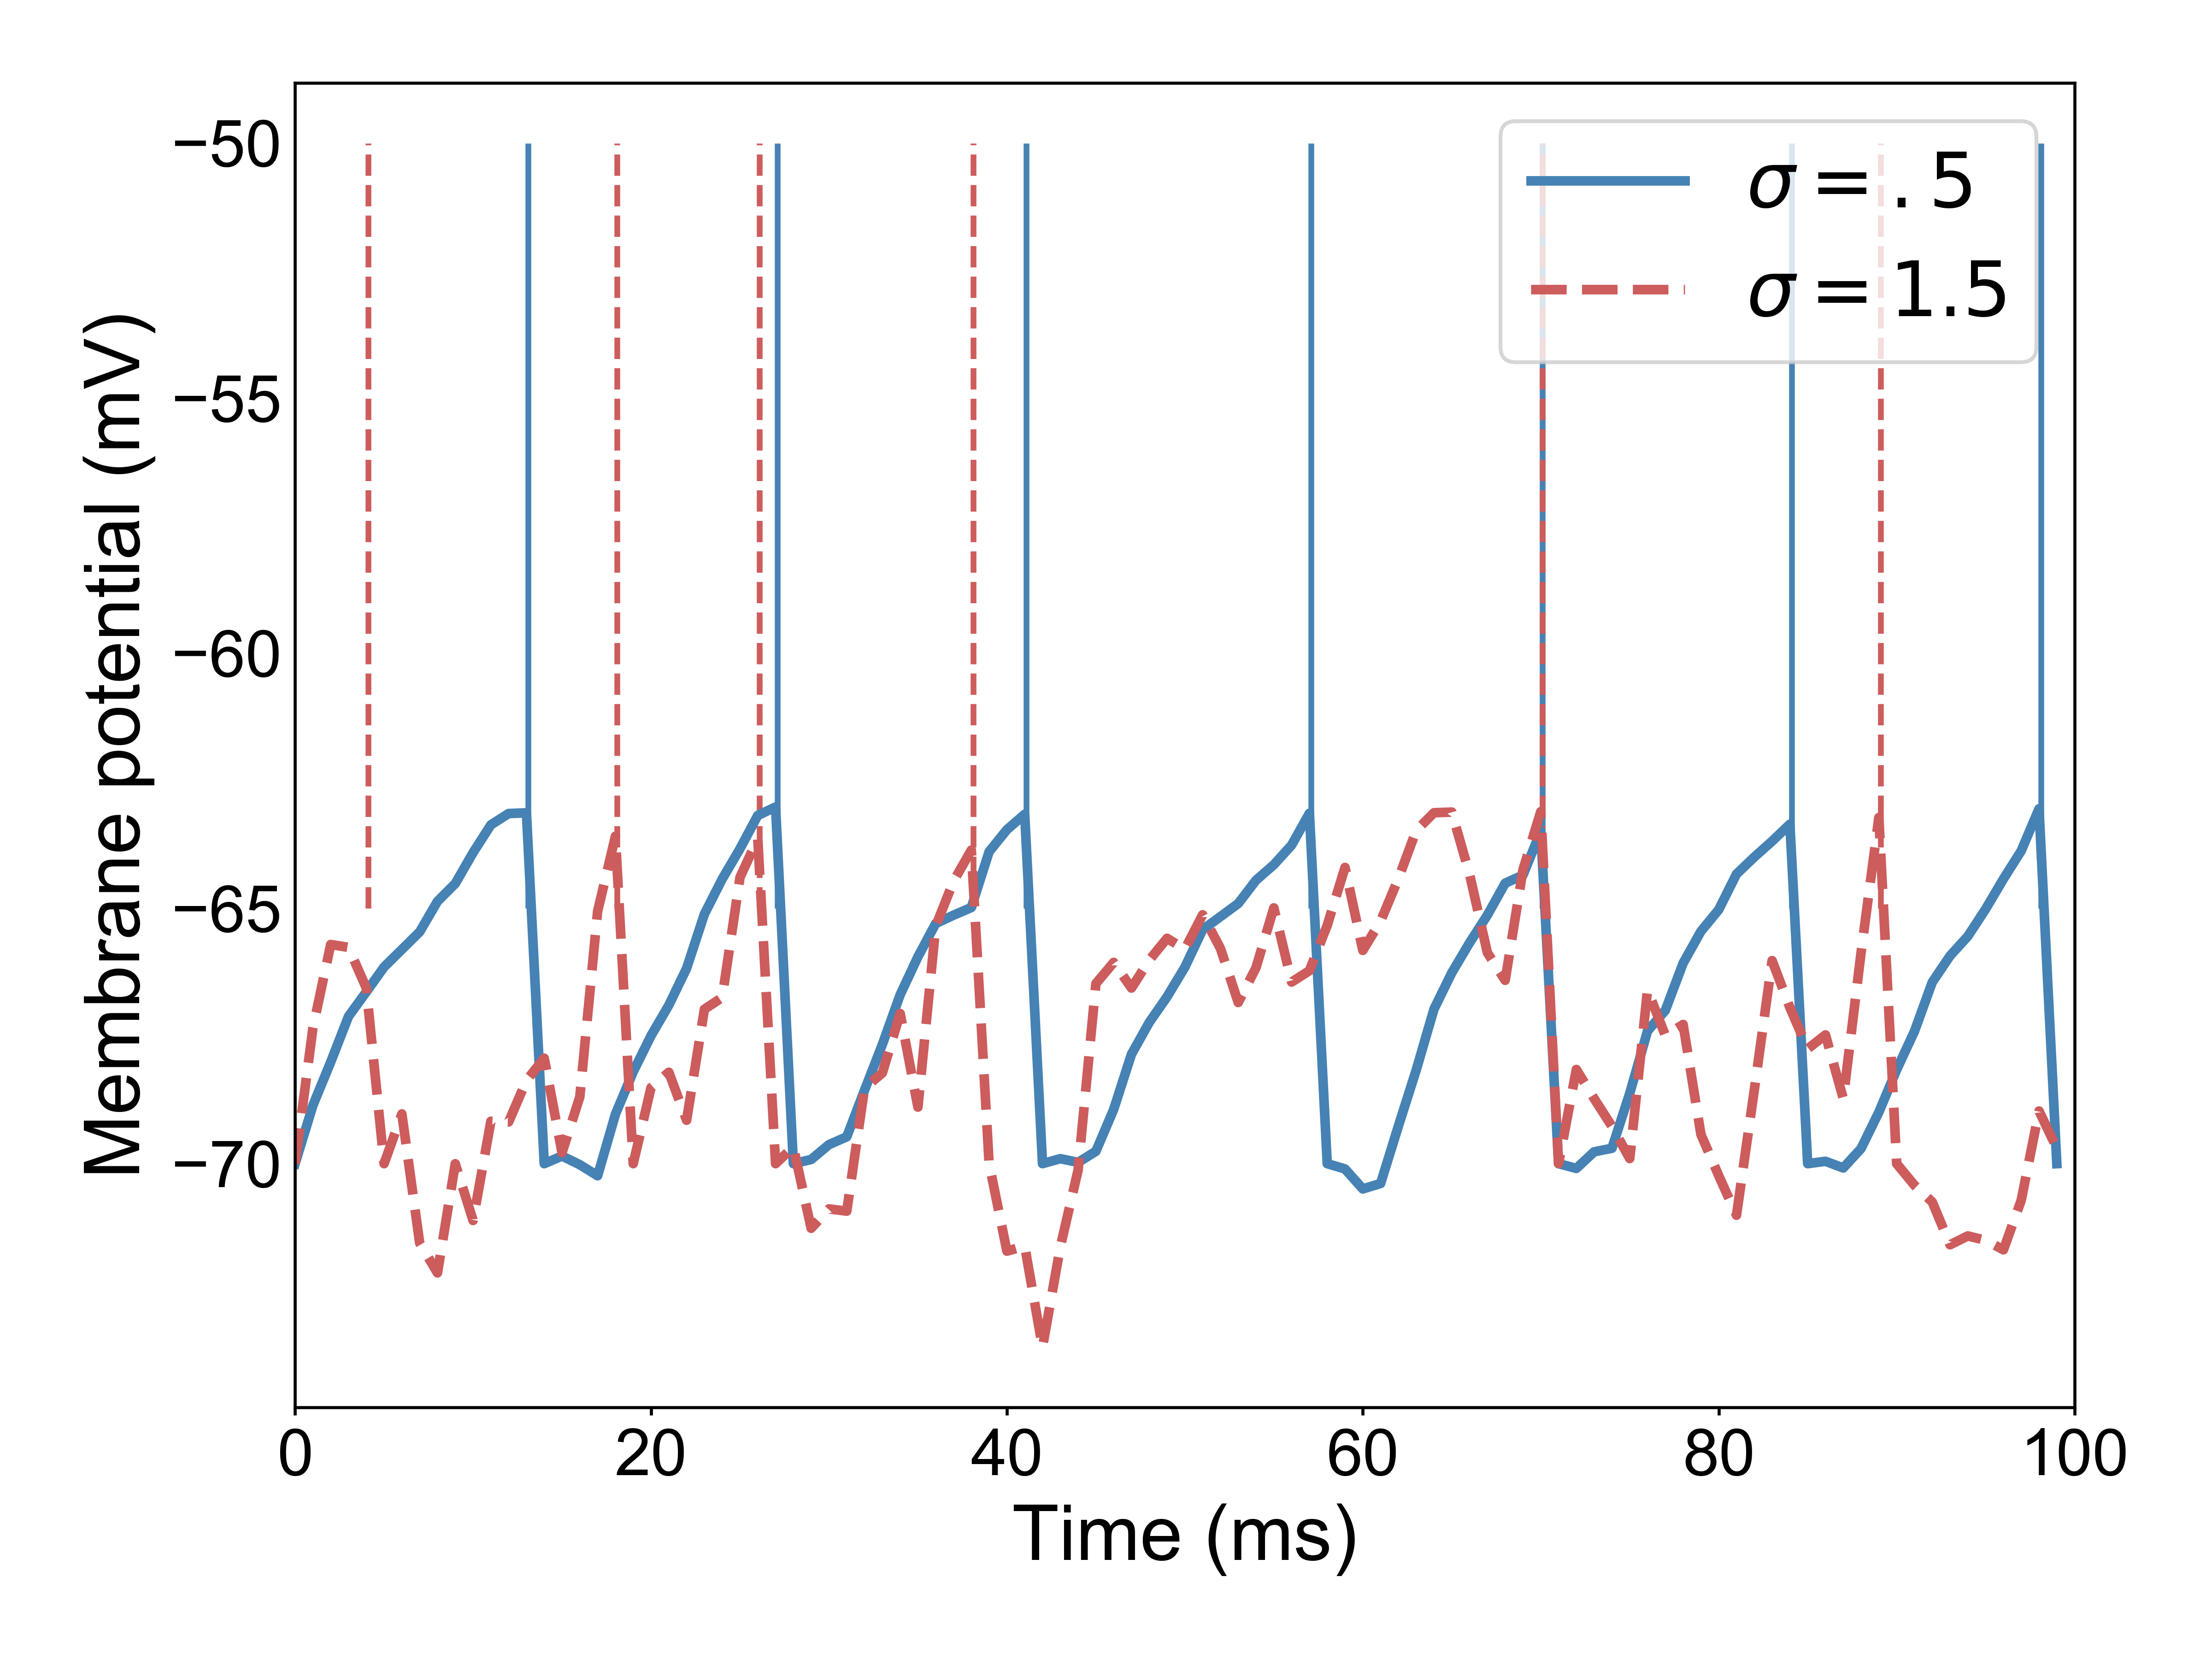
\includegraphics[width=0.8\linewidth]{report3_fig12.png}
\caption[growing population]{Membrane potential V(t) in time, with an injected current I=1, with a reset mechanism added, a refractory period RP=3, and different weights given to the noise.}\label{fig:fig9}
\end{figure}

With all these characteristics added to our model, we can easily reproduce the behavior the monkey's neurons exhibited in section \ref{ana}. Let create a current array I, such that I transiently increase during the 500 ms of stimulation, every $\frac{1000}{\text{frequency}}$ ms. Moreover, to be (artificially) closer to the original data that had $\Delta t = 5$ ms, let RP=5.\\
Several simulations showed that good parameters for the model were $I_{no\_stim} = 0.1$ and $I_{stim}=3$, the increase should last 15 ms, and $\sigma=1.2$, as there was a significant amount of random spiking in the data. Figure \ref{fig:fig10} shows a result of such a simulation.

\begin{figure}[H]
\centering
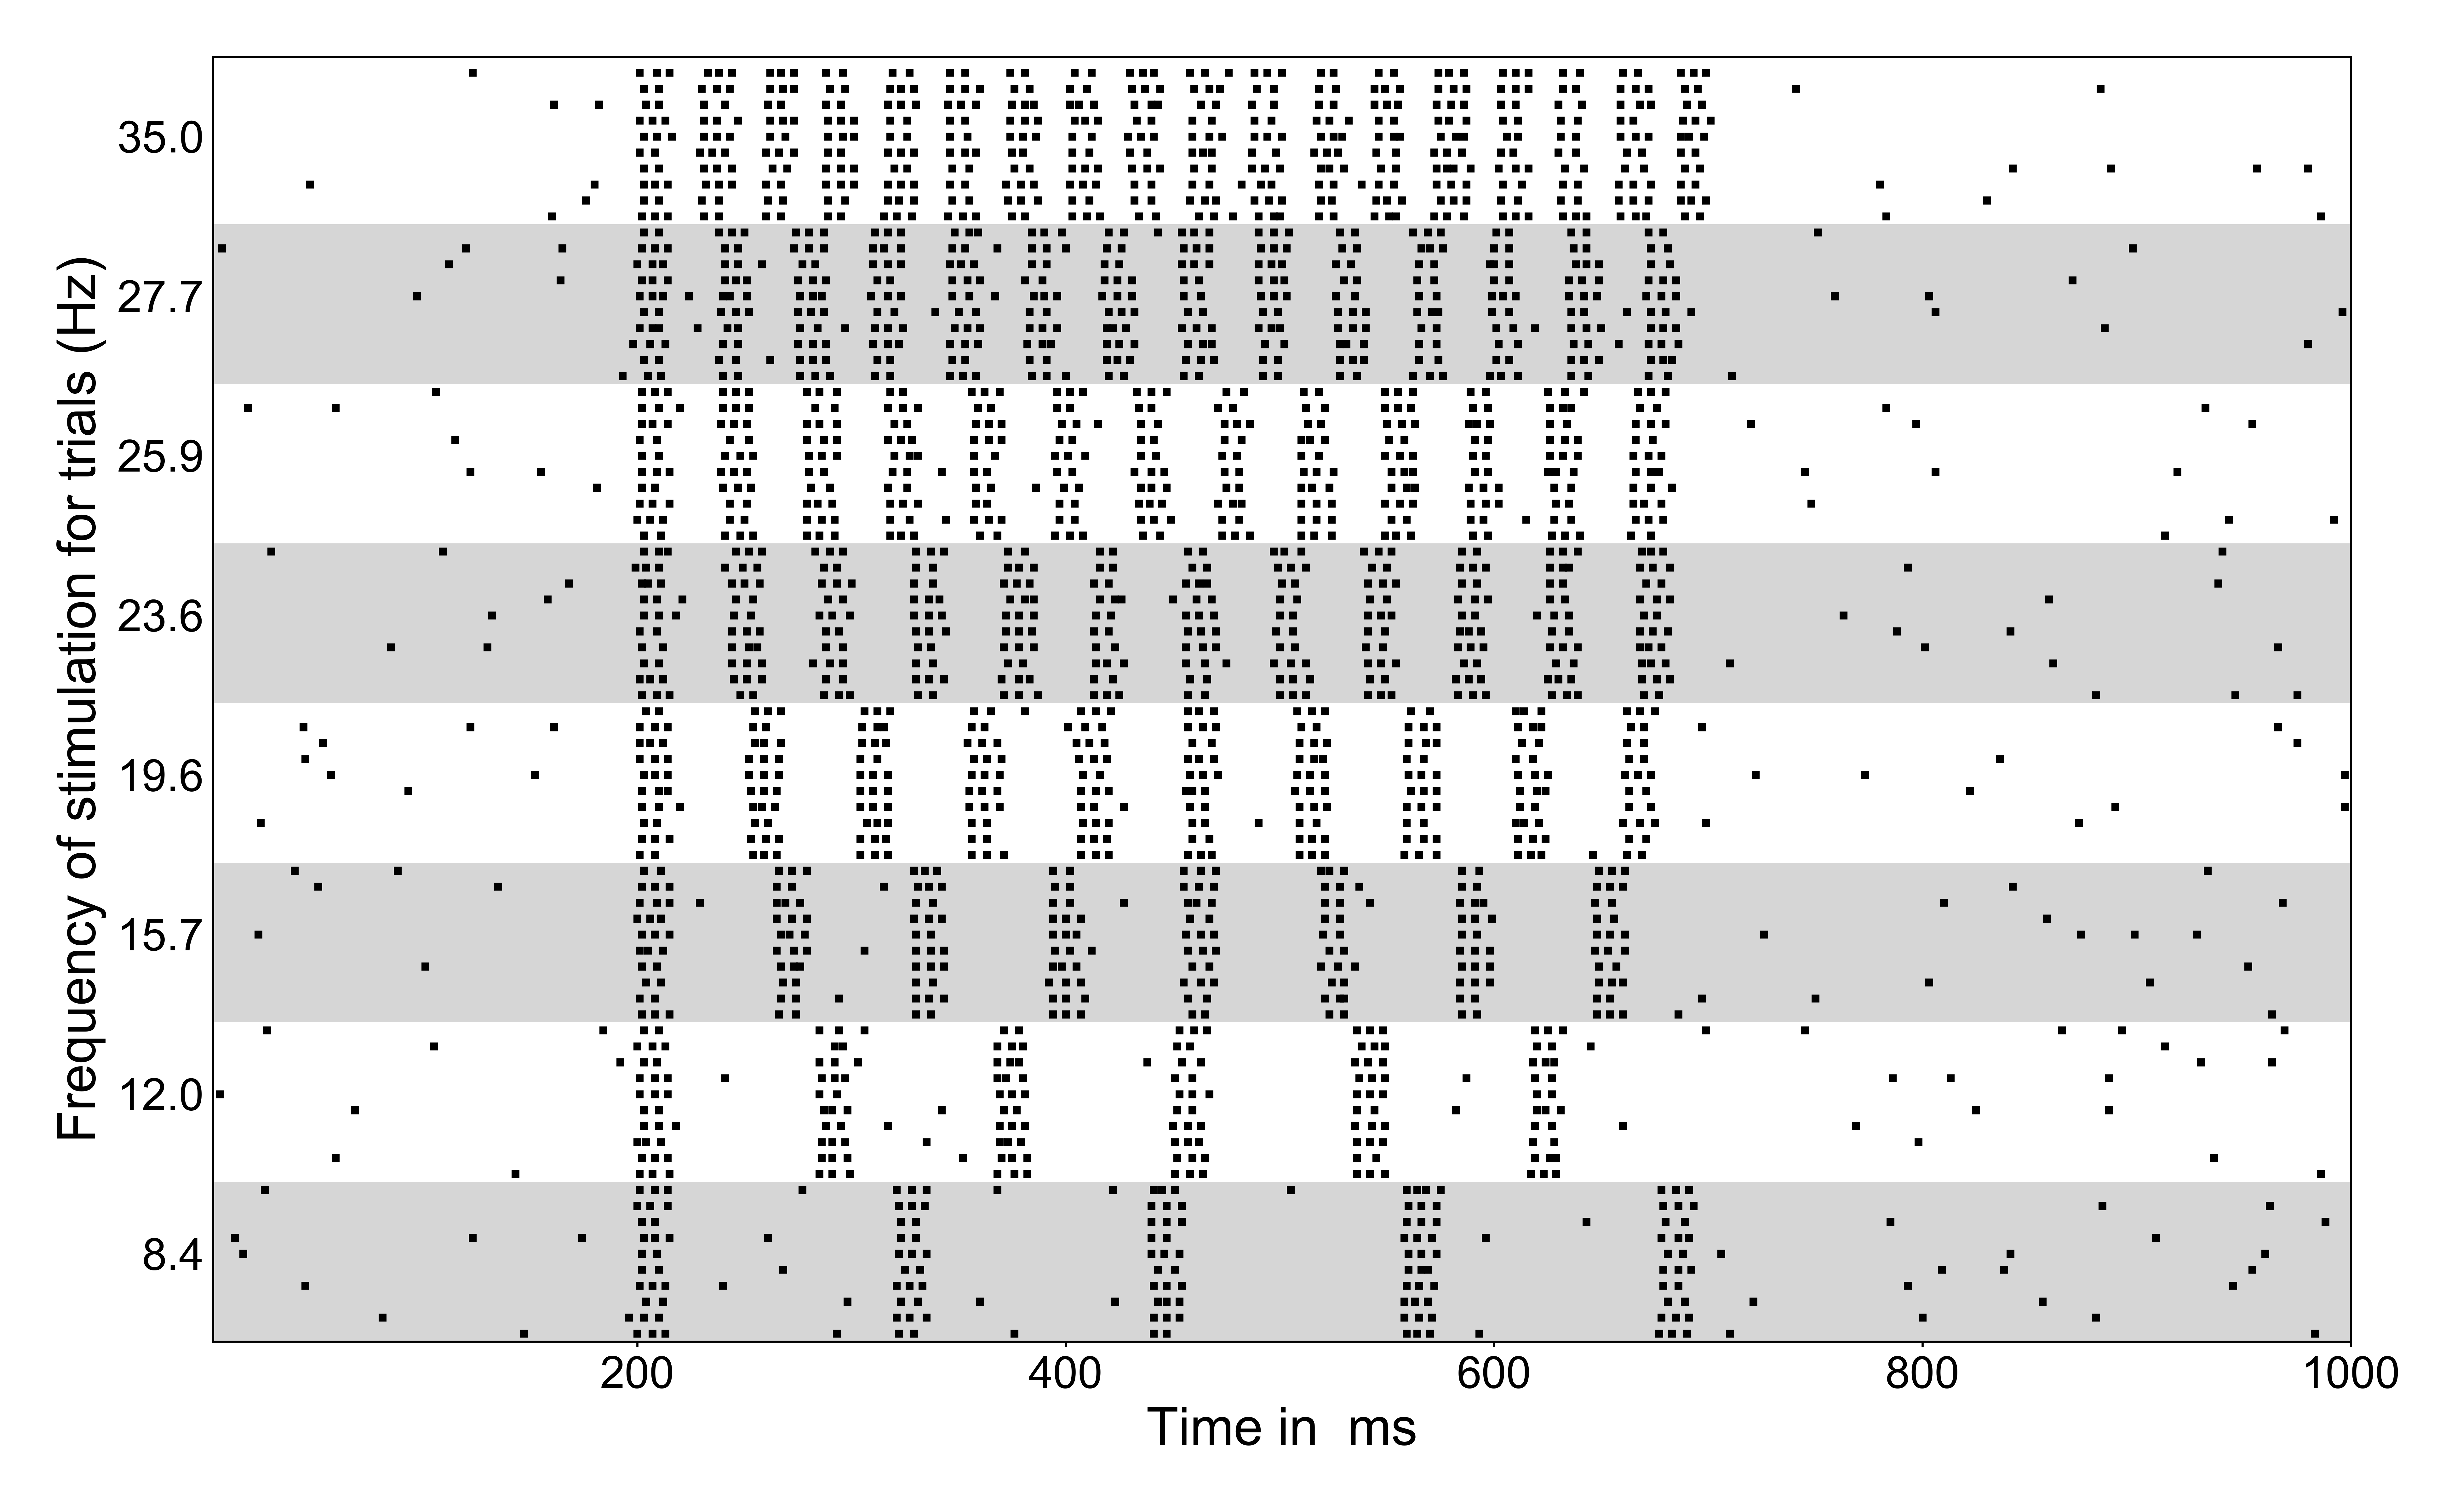
\includegraphics[width=1.1\linewidth]{report3_fig13.png}
\caption[growing population]{Spike trains of the modelled neuron at different frequency of stimulation (alternating current), for the parameters described above.}\label{fig:fig10}
\end{figure}

\section{Conclusion}
Cognitive neuroscience tries to relate brain activity to behavior, for instance by looking at the electrical activity of neurons in animals. The most meaningful part of this activity is the spikes, that can even directly `encode' external stimuli. However, the spiking activity of neurons is really stochastic, and the best way to make sense of spike trains, is to average them over many trials, to get a mean firing rate. A single spike train doesn't necessary bring a lot of information, but a firing rate can (see section \ref{ana})\\

Random spikes appearing at an interval determined by a firing rate are easy to simulate, but they don't really model a neuron's behavior. However, it is not so complicated to simulate the polarisation of the cell membrane, as it is a RC circuit. And, using real parameters measured experimentally (capacitance, resitance, equilibrium potential and refractory period), the model can be a pretty good biophysical description of a real neuron, and exhibit similar behavior, up to a certain point. Indeed, to really observe spiking activity in response to injected currents, one must artificially add features: a threshold after which the neuron spike and its membrane potential is reset to the equilibriumm potential, and gaussian noise.\\

Nevertheless, as efficient the model is, it doesn't take into account all the different ion flows through different types of channels that generate this potential. And this part can be especially important while studying pathologies, in which channel properties are often altered, thus causing atypical behavior. The Hodgkin-Huxley model tries to account for each channel type (as the opening of a single channel is very stochastic), and can be helpful at the single neuron level. However, with several neurons, it can be rapidly hard to interpret, and the LIF model is a good alternative.



\end{document}
